\documentclass[aspectratio=169, usenames,dvipsnames, 14pt]{beamer}
\usepackage[utf8]{inputenc}
\usepackage[utf8]{inputenc}
\usepackage{multirow}
\usepackage{gensymb}
\usepackage[absolute,overlay]{textpos}
\usepackage[export]{adjustbox}
\usepackage[absolute,overlay]{textpos}  % Absolute placement of text in frame

% \usepackage[dvipsnames]{xcolor} % Testing for color of slide 11
\usepackage{listings}           % For source code fonts
\usepackage{tikz}               % For absolute image placement and shapes
\usepackage{Formatting/python_formatting}   % User defined formatting file for source codes

% \usepackage{Formatting/grid_overlay}        % Grid overlay for accurate placement of images

\usetikzlibrary{calc}           % For absolute image placement
\usetikzlibrary{decorations.pathreplacing}      % For curly braces

\usetikzlibrary{arrows, positioning, shapes.geometric, quotes, angles}

\mode<presentation>
\usetheme{Rochester}


\title{\textbf{Getting Started With OpenMDAO}}
\author{Author Number One}

\begin{document}

%---------------------------------------------------------------------
\begin{frame}
    
    \maketitle

    \tikz[remember picture, overlay] \node[anchor=center] at ($(current page.center)-(5,1)$) {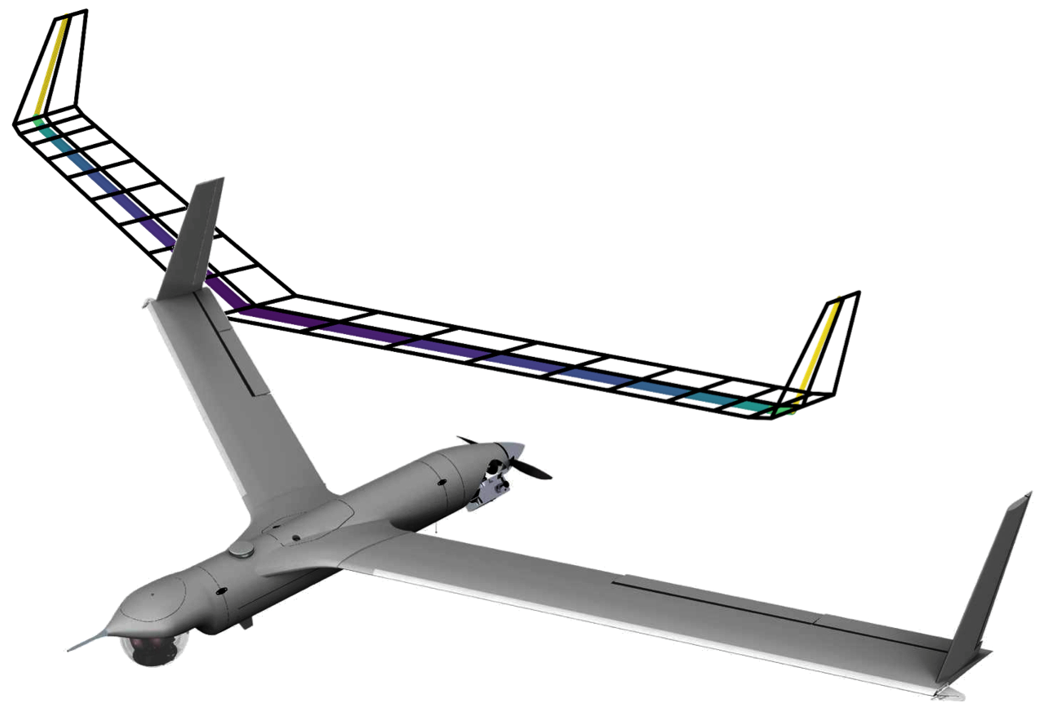
\includegraphics[scale=0.15]{images/frong2.png}};

    \tikz[remember picture, overlay] \node[anchor=center] at ($(current page.center)-(-5,1)$) {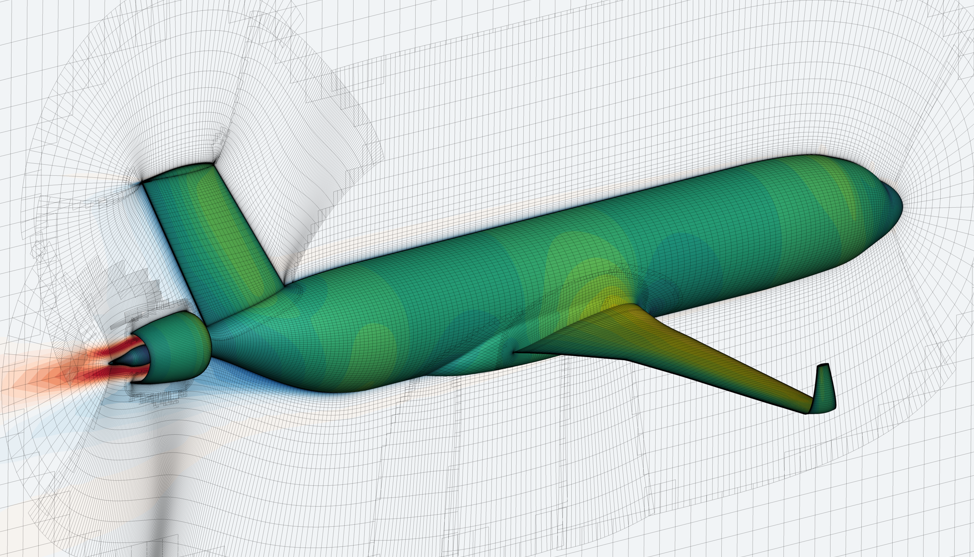
\includegraphics[scale=0.17]{images/front1.png}};

    \tikz[remember picture, overlay] \node[anchor=center] at ($(current page.center)-(0,-3.7)$) {
\includegraphics[scale=0.24]{images/omdao.png}};

    \tikz[remember picture, overlay] \node[anchor=center] at ($(current page.center)-(-5,3.4)$) {
\includegraphics[scale=0.21]{images/michiganlogo.png}};

\end{frame}
%---------------------------------------------------------------------

\begin{frame}{Download these slides and tutorial scripts from GitHub}

    \centering
    \url{https://github.com/johnjasa/openmdao\_training}

\end{frame}
%---------------------------------------------------------------------


%\begin{frame}{Acknowledgements}
%    \begin{itemize}
%        \item \textbf{Ben Brelje}, PhD candidate at University of Michigan MDO Lab for creating version 0 of this 
%        \vspace{0.5cm}
%        \item \textbf{Justin Gray}, Engineer and team lead of OpenMDAO at NASA Glenn for refining this workshop
%        \vspace{0.5cm}
%        \item NASA ARMD’s TTT Project has supported OpenMDAO development since 2008
%    \end{itemize}
%    
%\end{frame}
%---------------------------------------------------------------------

\begin{frame}{Dymos is an open-source library for modeling dynamic systems within OpenMDAO}
    \begin{itemize}
        \item Support for multiple optimal control techniques
        \vspace{0.25cm}
        \item Doesn't impose the trajectory optimization as the ``top-level'' problem
        \vspace{0.25cm}
        	\begin{itemize}
        	  \item Treats the trajectory as on component of a larger system
    		  \vspace{0.25cm}
		      \item Design a system to satisfy multiple design reference trajectories
		    \end{itemize}
        \vspace{0.25cm}
		\item Find the best system to fly a trajectory, and the best trajectory that can be flown by the system
    \end{itemize}
\end{frame}

\begin{frame}{Dymos is an open-source library for modeling dynamic systems within OpenMDAO}
    \begin{itemize}
        \item Support for multiple optimal control techniques
        \vspace{0.25cm}
        \item Doesn't impose the trajectory optimization as the ``top-level'' problem
        \vspace{0.25cm}
        	\begin{itemize}
        	  \item Treats the trajectory as on component of a larger system
    		  \vspace{0.25cm}
		      \item Design a system to satisfy multiple design reference trajectories
		    \end{itemize}
        \vspace{0.25cm}
		\item Find the best system to fly a trajectory, and the best trajectory that can be flown by the system
    \end{itemize}
\end{frame}
%---------------------------------------------------------------------


\begin{frame}{Dymos leverages the strengths of OpenMDAO}
    \begin{itemize}
        \item Analytic derivatives and automatic detection of sparsity patterns
        \vspace{0.25cm}
        	\begin{itemize}
        	  \item Adjoint differentiation tends to be faster for shooting methods
              \vspace{0.25cm}
        	  \item Pseudospectral methods tend to be faster in forward mode
              \vspace{0.25cm}
	  		  \item Bidirectional sparsity for problems which would ``break'' pure forward or reverse sparsity
	        \end{itemize}
        \vspace{0.25cm}
		\item Parallelization of expensive models via MPI
        \vspace{0.25cm}
        \item Access to OpenMDAO solvers within the ODE
    \end{itemize}
\end{frame}


\begin{frame}{Dymos Numerical Methods}
    \begin{itemize}
	  	\item Pseudospectral methods
		\vspace{0.25cm}
		    \begin{itemize}
		      \item High-Order Gauss-Lobatto (OTIS)
    		  \vspace{0.25cm}
		      \item Radau Pseudospectral Method (GPOPS, DIDO)
		    \end{itemize}
        \vspace{0.25cm}
        \item Shooting methods
        \vspace{0.25cm}
        	\begin{itemize}
        	  \item RK4
	          \vspace{0.25cm}
	          \item Solver-based pseudospectral methods
	        \end{itemize}
    \end{itemize}
\end{frame}


\begin{frame}{Dymos Numerical Methods}
    \begin{itemize}
	  	\item Pseudospectral methods
		\vspace{0.25cm}
		    \begin{itemize}
		      \item High-Order Gauss-Lobatto (OTIS)
    		  \vspace{0.25cm}
		      \item Radau Pseudospectral Method (GPOPS, DIDO)
		    \end{itemize}
        \vspace{0.25cm}
        \item Shooting methods
        \vspace{0.25cm}
        	\begin{itemize}
        	  \item RK4
	          \vspace{0.25cm}
	          \item Solver-based pseudospectral methods
	        \end{itemize}
    \end{itemize}
\end{frame}


\begin{frame}{The problem solved by Dymos}
    \begin{itemize}
	  	\item Minimize/maximize some objective quantity subject to:
		\vspace{0.25cm}
		    \begin{itemize}
		      \item Dynamics (provided by an OpenMDAO system)
    		  \vspace{0.25cm}
		      \item Dynamic controls
    		  \vspace{0.25cm}
		      \item Static Controls (design parameters)
    		  \vspace{0.25cm}
		      \item Boundary Constraints
    		  \vspace{0.25cm}
		      \item Path Constraints
		    \end{itemize}
    \end{itemize}    
\end{frame}


\begin{frame}{The Dymos UI is heavily influenced by OTIS}
    \begin{itemize}
	  \item A \emph{trajectory} is broken into one or more \emph{phases}
	  \item In each \emph{phase} states and controls are represented on one or more polynomial \emph{segments} in time
	  \item Phases can be linked via constraint (supports parallel execution) or connected in series
	  \item Phase linkages are very general, supporting branched trajectories
	\end{itemize}
\end{frame}


\begin{frame}{Notable features of Dymos}
    \begin{itemize}
	  \item Vectorized states, controls, and parameters
	  \vspace{0.25cm}
	  \item Access to the first and second time derivatives of controls
	  \item Output available on arbitrary grids
	\end{itemize}
\end{frame}
%---------------------------------------------------------------------

\begin{frame}{Goals for today}
    \begin{itemize}
        \item Solve an optimal control problem with Dymos
        \vspace{.5cm}
        \item Learn what to do when things don't go well
        \vspace{.5cm}
        \item Get \textcolor{red}{\textbf{really excited}} about using analytic derivatives for optimization!

    \end{itemize}
    
\end{frame}
%---------------------------------------------------------------------

\begin{frame}{Dymos by Example}
    \begin{block}{The Enemy Submarine Problem}
      \footnotesize
      An enemy submarine determined to sink your ship is sitting, torpedoes armed, exactly halfway between you and your home port. The submarine submerges to some fixed depth, and your ship now has no further information about its position. The enemy sub has to be directly underneath your ship to sink it, but the sub can track your moves with precision and respond efficiently. If your ship is fast enough, though, you will be able to set a wide course around the sub and reach port safely.\\
\vspace{1em}
How much faster than the sub does your ship have to be to guarantee you can avoid the sub and get home?\\
    \end{block}
    
    \tiny
    Source: \url{https://fivethirtyeight.com/features/damn-the-torpedoes-two-puzzles-ahead/}
\end{frame}

\begin{frame}{The Enemy Submarine Problem: ODE}

    \begin{columns}[T]
    \column{0.3 \textwidth}

        \begin{tikzpicture}[semithick,scale=2]
            \tikzstyle{subj} = [circle, minimum width=8pt, fill, inner sep=0pt]
            \tikzstyle{empty}  = [circle, minimum width=8pt, inner sep=0pt]
            \tikzstyle{dc}   = [circle, minimum width=8pt, draw, inner sep=0pt, path picture={\draw (path picture bounding box.south east) -- (path picture bounding box.north west) (path picture bounding box.south west) -- (path picture bounding box.north east);}]

            \tikzstyle{every label}=[font=\bfseries]

            % Before diagram .........................
            \node[subj,  label=below:o] (o) at (0,0) {};
            \node[empty, label=above:$\hat{j}$] (y) at (0,2) {};
            \node[empty, label=right:$\hat{i}$] (x) at (2,0) {};
            \node[empty, label=below:$v$] (v) at (1.68,1.08) {};

            \draw[->] (o) -- (y);
            \draw[->] (o) -- (x);
            \draw[->] (o) -- (v);

            \draw pic["$\phi$",draw=black,<->,angle eccentricity=1.2,angle radius=1cm] {angle=v--o--y};

        \end{tikzpicture}

    \column{0.3 \textwidth}
        \begin{align*}
            \dot{x} &= v \sin{\phi} \\
            \dot{y} &= v \cos{\phi}
        \end{align*}
\end{columns}

\end{frame}

\begin{frame}{The Enemy Submarine Problem: ODE}
    \begin{itemize}
      \item Give the sub a speed of 1 (unitless).
      \item The sub can, at best, be $time$ units in distance away from its starting point
      \begin{align*}
      r_{sub} = time
      \end{align*}
    \end{itemize}
\end{frame}

\begin{frame}{The Enemy Submarine Problem: ODE}
    \begin{itemize}
      \item Path constraint:  To avoid the sub, our ship must be greater than $r_{sub}$ units away from its origin at any given time.
      \begin{align*}
      r_{ship} &= \sqrt{x^2 + y^2}\\
      r_{ship} - r_{sub} &\ge 0
      \end{align*}
    \end{itemize}
\end{frame}


\begin{frame}{The Donner Sub Problem: Notional XDSM}
    \centering
    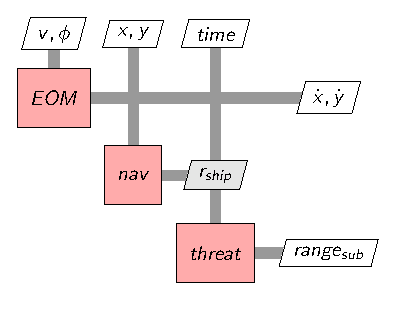
\includegraphics[scale=1.0]{images/donner_sub/donner_sub_ode_xdsm}
\end{frame}

\begin{frame}{The Donner Sub Problem: ODE}


    \lstset{basicstyle=\tiny}
    \lstinputlisting[language=Python]{SourceCodes/donner_sub/1/donner_sub_ode.py}

    \pause
  
    \only<2>{
        \begin{tikzpicture}[overlay]
            \draw[red, very thick, ->] (8.5cm,3.75cm) to (7.1cm, 3.75cm);
        \end{tikzpicture}
  
        \begin{textblock*}{6cm}(9.75cm,4.7cm)
            \footnotesize \textcolor{red}{All ODE models accept num\_nodes}
        \end{textblock*}
  }
  
  \pause
  
    \only<3>{
        \begin{tikzpicture}[overlay]
            \draw[red, very thick, ->] (6.2cm,1.50cm) to (7.2cm, 1.50cm);
        \end{tikzpicture}

        \begin{textblock*}{7cm}(1.5cm,7.0cm)
            \footnotesize \textcolor{red}{Size ExecComp variables appropriately}
        \end{textblock*}
  }

\end{frame}     % Error is from the source code being outside the defined area (can ignore)


\begin{frame}{Setting up the problem}
    \begin{itemize}
      \item One phase (single ODE, no intermediate boundary constraints)
      \item Two state variables ($x$, $y$)
      \item One design parameter ($v$)
      \item One dynamic control ($\phi$)
      \item Objective: minimize $v$
    \end{itemize}
\end{frame}


%
%%---------------------------------------------------------------------
%\begingroup
%\setbeamercolor{background canvas}{bg=GreenYellow}
%\begin{frame}{OpenMDAO intro and Basics}
%
%    \begin{itemize}
%        \item Intro and terminology
%        \vspace{0.5cm}
%        \item Building explicit components and connecting them together
%        \vspace{0.5cm}
%        \item Lab 0: Implementing a simple explicit calculation (Breguet Range)
%    \end{itemize}
%
%\end{frame}
%\endgroup
%%---------------------------------------------------------------------
%
%\begin{frame}{OpenMDAO has nice features}
%    \begin{itemize}
%        \item Units
%          \begin{itemize}
%              \item Conversions
%              \item (In)compatibility checks
%          \end{itemize}
%\pause
%\vspace{.5cm}
%        \item Automatic checks for unconnected inputs
%\pause
%\vspace{.5cm}
%        \item Interactive N2 diagrams
%\pause
%\vspace{.5cm}
%        \item Models are Python objects (inheritance!)
%    \end{itemize}
%\end{frame}
%%---------------------------------------------------------------------
%
%\begin{frame}{OpenMDAO has best-in-class numerical methods}
%    \begin{itemize}
%        \item Efficient solvers for implicit systems
%        \begin{itemize}
%            \item Newton solver
%            \item Nonlinear block Gauss-Seidel
%        \end{itemize}
%\pause
%\vspace{0.5cm}
%        \item Derivative computation (for gradient-based opt.)
%        \begin{itemize}
%            \item Forward and reverse analytic
%            \item Finite difference or complex step
%            \item Mixture of all!
%            \end{itemize}
%\pause
%\vspace{0.5cm}
%        \item MPI parallelization
%    \end{itemize}
%
%\end{frame}
%%---------------------------------------------------------------------
%
%\begin{frame}{OpenMDAO architecture}
%\begin{columns}[T]
%    \column{0.5 \textwidth}
%        \begin{itemize}
%            \item \textbf{Components} implement the actual model computation
%        \vspace{0.5cm}
%            \uncover<2->{\item Groups organize the model and enable hierarchical solver strategies}
%        \vspace{0.5cm}
%            \uncover<3->{\item Drivers iteritively execute the model (optimizers and DOEs)}
%        \vspace{0.5cm}
%            \uncover<4->{\item \textbf{Problem} is the top-level container}
%        \end{itemize}
%
%    \column{0.5 \textwidth}
%        \uncover<1->{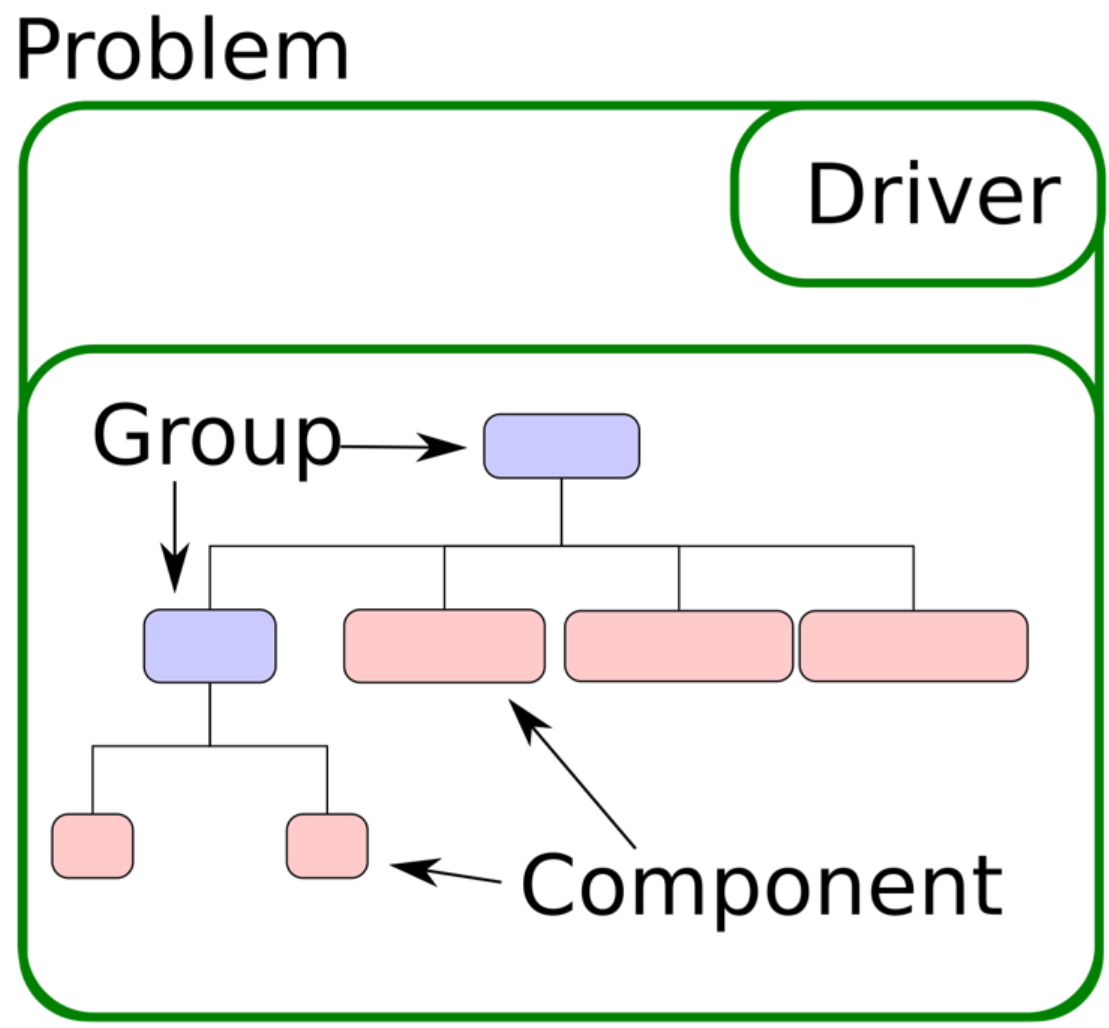
\includegraphics[scale=0.2]{images/arch1.png}}
%\end{columns}
%
%\end{frame}
%%---------------------------------------------------------------------
%
%\begin{frame}{ExplicitComponent class}
%%    \begin{columns}[T]
%%
%%        \column{0.5 \textwidth}
%%            \begin{itemize}
%%                \item Used for doing explicit calculations
%%                \vspace{.5cm}
%%                \uncover<2->{\item Inputs $\rightarrow$ Outputs with no iteration / implicit states}
%%                \vspace{.5cm}
%%                \uncover<3->{\item Can be as simple as a one-line calculation, or as complex as an adjoint CFD solver}
%%            \end{itemize}
%%
%%    \column{0.5 \textwidth}
%%        \begin{tikzpicture}[overlay]
%%            \draw (2.9, -2) node [inner sep=0] {\uncover<1->{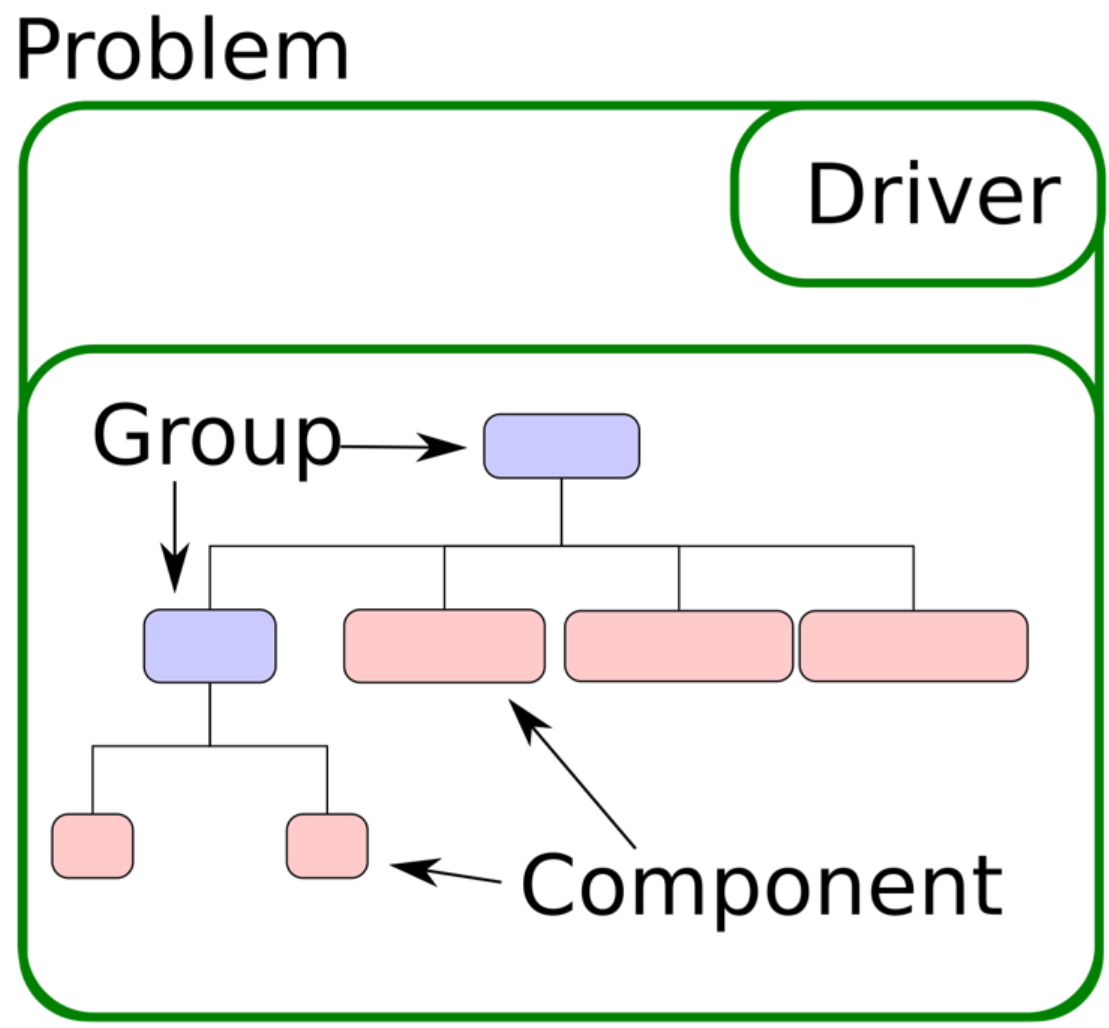
\includegraphics[scale=0.2]{images/arch1.png}};}
%%            \draw [blue, ultra thick] (4.8,-2.7) circle (0.65cm);
%%            \draw[blue, very thick] (-2,1.3) -- (4.2, -2.5);
%%        \end{tikzpicture}
%%  \end{columns}
%
%\end{frame}
%%---------------------------------------------------------------------
%% Need to have alternating white/grey lines in background
%\begin{frame}{The Donner Sub Problem: ODE}
%
%
%    \lstset{basicstyle=\tiny}
%    \lstinputlisting[language=Python]{SourceCodes/donner_sub_ode.py}
%
%    \pause
%
%    \only<2>{
%        \begin{tikzpicture}[overlay]
%            \draw[red, very thick, <-] (7.1cm,5.7cm) to (8.5cm, 5.7cm);
%        \end{tikzpicture}
%
%        \begin{textblock*}{6cm}(9.75cm,3.75cm)
%            \footnotesize \textcolor{red}{All ODE models accept num\_nodes}
%        \end{textblock*}
%  }
%
%  \pause
%
%    \only<3>{
%        \begin{tikzpicture}[overlay]
%            \draw[red, very thick, <-] (10.6cm,5.4cm) to (11.5cm, 5.8cm);
%        \end{tikzpicture}
%
%        \begin{textblock*}{6cm}(9.3cm,2.35cm)
%            \footnotesize \textcolor{red}{Define any options / run flags which\\do not change during evaluation}
%        \end{textblock*}
%    }
%
%  \pause
%
%    \only<4>{
%        \begin{tikzpicture}[overlay]
%            \draw[red, very thick, <-] (10.6cm,4.4cm) to (11.5cm, 5.8cm);
%        \end{tikzpicture}
%
%        \begin{textblock*}{7cm}(8.5cm,2.2cm)
%            \footnotesize \textcolor{red}{Define model inputs, output, and (optionally)\\partial derives using the setup() method.\\Called once before solve / optimization}
%        \end{textblock*}
%  }
%
%  \pause
%
%    \only<5>{
%        \begin{textblock*}{7cm}(9cm,6.6cm)
%            \footnotesize \textcolor{red}{Do the actual computation using compute(). Need to fill in values for all your declared outputs by the end of this method. Called every time the model is evaluated}
%        \end{textblock*}
%  }
%
%  \pause
%
%    \only<6>{
%%----------------------------------------------------------------------------------------
%%----------Begin the arrows and text on the last 'ExplicitComponent example' Frame-------
%%----------------------------------------------------------------------------------------
%        \begin{tikzpicture}[overlay]
%            \draw[red,very thick, <-](4.2cm,4.3cm) to (5.8cm,6.5cm);
%        \end{tikzpicture}
%
%        \begin{textblock*}{5cm}(7cm,2.3cm)
%            \footnotesize \textcolor{red}{Variable name}
%        \end{textblock*}
%%-------------%------------
%        \begin{tikzpicture}[overlay]
%            \draw[red,very thick, <-](5cm,4.3cm) to (7cm,6cm);
%        \end{tikzpicture}
%
%        \begin{textblock*}{5cm}(7.6cm,2.7cm)
%            \footnotesize \textcolor{red}{Default value (before model runs)}
%        \end{textblock*}
%%-------------%------------
%        \begin{tikzpicture}[overlay]
%            \draw[red,very thick, <-](6.2cm,4.3cm) to (8cm,5.6cm);
%        \end{tikzpicture}
%
%        \begin{textblock*}{5cm}(9cm,3.1cm)
%            \footnotesize \textcolor{red}{Units (need not match upstream)}
%        \end{textblock*}
%%-------------%------------
%        \begin{tikzpicture}[overlay]
%            \draw[red,very thick, <-](8.8cm,4.4cm) to (10.9cm,4.8cm);
%        \end{tikzpicture}
%
%        \begin{textblock*}{3cm}(12.3cm,3.7cm)
%            \footnotesize \textcolor{red}{Human-readable description (optional)}
%        \end{textblock*}
%%-------------%------------
%        \begin{tikzpicture}[overlay]
%            \draw[red,very thick, <-](8.2cm,2.8cm) to (11.4cm,3.1cm);
%        \end{tikzpicture}
%
%        \begin{textblock*}{3cm}(12.8cm,5.7cm)
%            \footnotesize \textcolor{red}{Variable dimension (in this case, a n x 1 vector)}
%        \end{textblock*}
%        %-------------%------------
%        \begin{tikzpicture}[overlay]
%            \draw[red,very thick, <-](6.2cm,2cm) to (8cm,2cm);
%        \end{tikzpicture}
%
%        \begin{textblock*}{3.6cm}(9.5cm,7.2cm)
%            \footnotesize \textcolor{red}{Will default to expecting user provided analytic derivatives, but we can specify `fd` later…}
%        \end{textblock*}
%  }
%\end{frame}     % Error is from the source code being outside the defined area (can ignore)
%%---------------------------------------------------------------------
%
%\begin{frame}{Connecting multiple components}
%\begin{columns}
%    \column[T]{0.5\textwidth}
%        \begin{itemize}
%            \item Combine components into a Group to build models
%            \vspace{0.5cm}
%            \item Groups can hold other Groups, forming a hierarchy
%        \end{itemize}
%
%    \column[T]{0.5\textwidth}
%        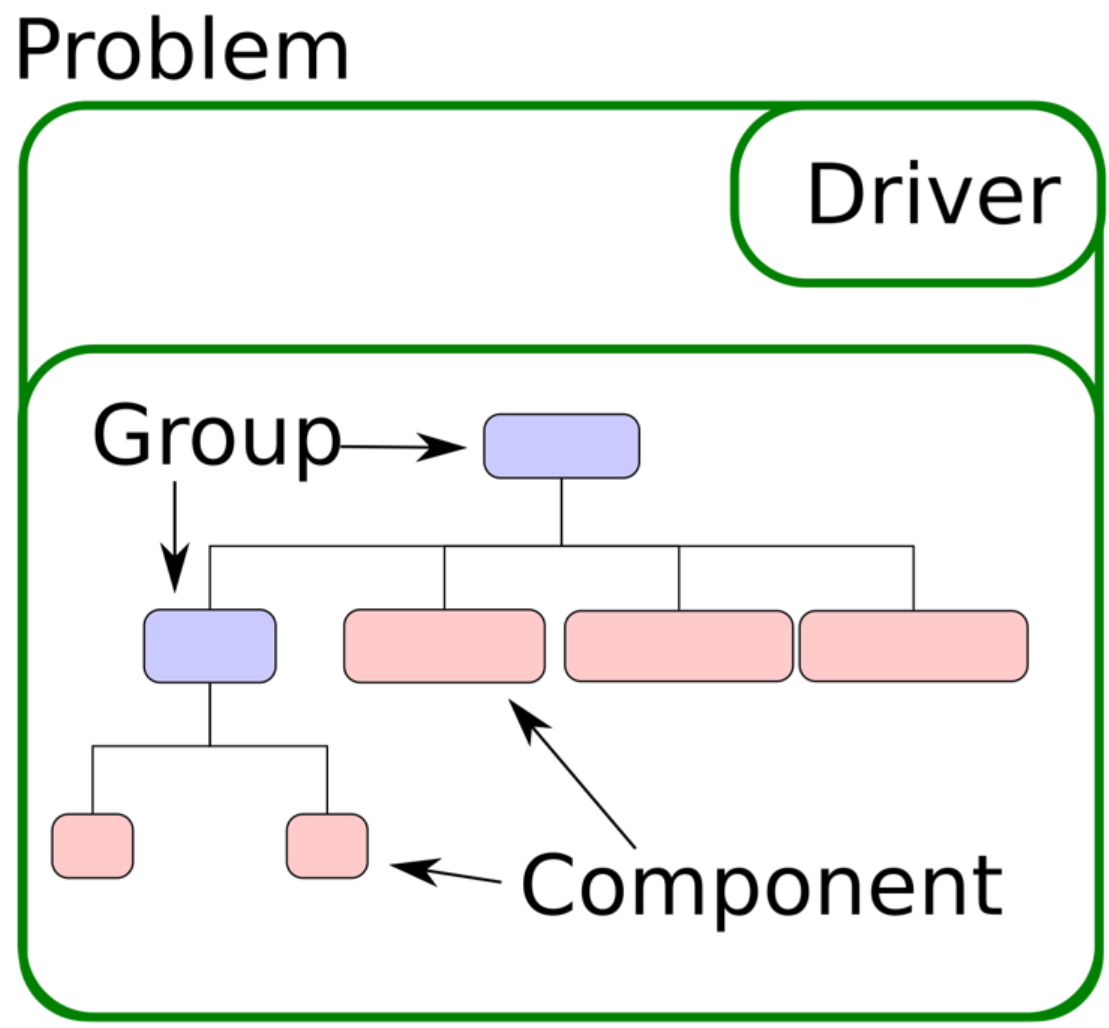
\includegraphics[scale=0.2]{images/arch1.png}
%        \begin{tikzpicture}[overlay]
%            \draw [blue, ultra thick] (-4.75,2) circle (0.55cm);
%      \end{tikzpicture}
%    \end{columns}
%
%\end{frame}
%%---------------------------------------------------------------------
%
%\begin{frame}{Connecting multiple components}
%    \lstinputlisting[language=Python]{SourceCodes/connecting_multiple_components.py}
%
%    \only<1>{
%        \begin{textblock*}{6cm}(8cm,2.7cm)
%            \footnotesize \textcolor{red}{Define a model by subclassing Group}
%        \end{textblock*}
%
%        \begin{tikzpicture}[overlay]
%            \draw[red,very thick,<-](3.9,6.35) to (6.7,6.25);
%        \end{tikzpicture}
%
%        \begin{textblock*}{5cm}(8.3cm,7cm)
%            \footnotesize \textcolor{red}{This is the model structure that is being connected}
%        \end{textblock*}
%
%        \begin{tikzpicture}[overlay]        % Curly brace
%            \draw [red, very thick,decorate,decoration={brace,amplitude=10pt,mirror,raise=4pt},yshift=0pt]
%            (6.2,2.3) -- (6.2,3.9) node [midway,xshift=3cm] {\footnotesize $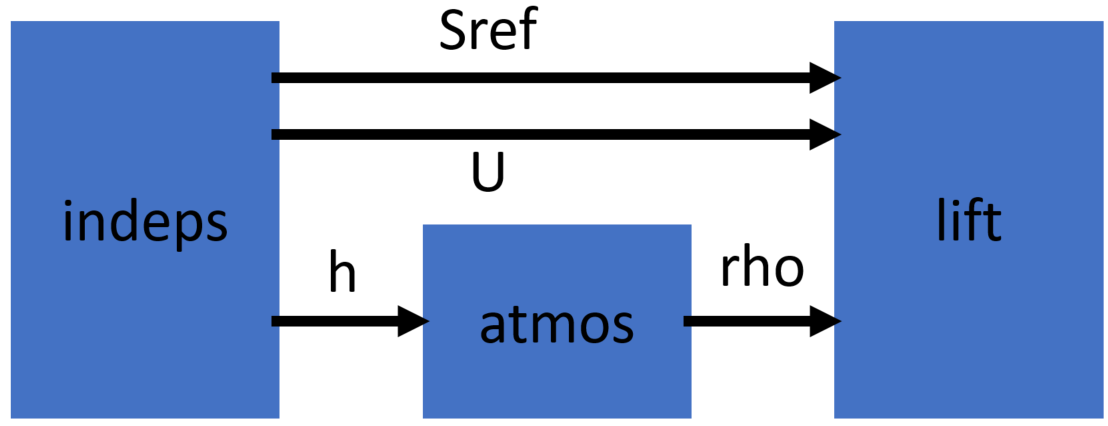
\includegraphics[scale=0.2]{images/explicit_box.png}$};
%        \end{tikzpicture}
%    }
%
%    \pause
%
%    \only<2>{
%%-------Puts grid on page to easily place textblocks and tikzpictures---------%
%% \begin{tikzpicture}[overlay]
%%   \draw [gray] (0,0) grid (15,9);
%% \end{tikzpicture}
%%-------------------------------%
%        \begin{tikzpicture}[overlay]
%            \draw[red, very thick, <-](4.6,5.8) to (8.5,5.2);         % Top Arrow
%            \draw[red, very thick] (4.6,4) rectangle ++(3.5,0.6);  % Box at line 11, 12
%            \draw[red, very thick,<-](7.9,4) to (10, 3.5);          % Bottom arrow
%        \end{tikzpicture}
%
%        \begin{textblock*}{5cm}(9.5cm,3.7cm)
%            \footnotesize \textcolor{red}{Include components using the add\_subsystem (name, component) method}
%        \end{textblock*}
%
%        \begin{textblock*}{4cm}(11cm,5.6cm)
%            \footnotesize \textcolor{red}{Python note: These are instances of a component class}
%        \end{textblock*}
%    }
%
%    \pause %----------------------------------------
%
%    \only<3>{
%        \begin{tikzpicture}[overlay]
%            \draw[red, very thick, <-](6.8,4.4) to (9,4.4);     %Top arrow
%            \draw[red, very thick, <-](6.8,4) to (10,2.5);        % Bottom arrow
%        \end{tikzpicture}
%
%        \begin{textblock*}{5cm}(10cm,3.8cm)
%            \footnotesize \textcolor{red}{Your custom components can be defined in the same .py file, or imported from a package for modularity}
%        \end{textblock*}
%
%        \begin{textblock*}{5cm}(11cm,7cm)
%            \footnotesize \textcolor{red}{Specify flags/options now}
%        \end{textblock*}
%    }
%
%    \pause %----------------------------------------
%
%    \only<4>{
%        \tikz[overlay]
%            \draw [red, very thick,decorate,decoration={brace,amplitude=10pt,mirror,raise=4pt},yshift=0pt]
%            (6.2,2.3) -- (6.2,3.9) node [midway,xshift=4.45cm] {};
%
%        \begin{textblock*}{5cm}(8cm,6.1cm)
%            \footnotesize \textcolor{red}{Connect parameters using the connect(from, to) method}
%        \end{textblock*}
%
%        \tikz[overlay]        % Connection boxes image
%            \node[anchor=center] at ($(current page.center)-(-3,-0.5)$)
%            {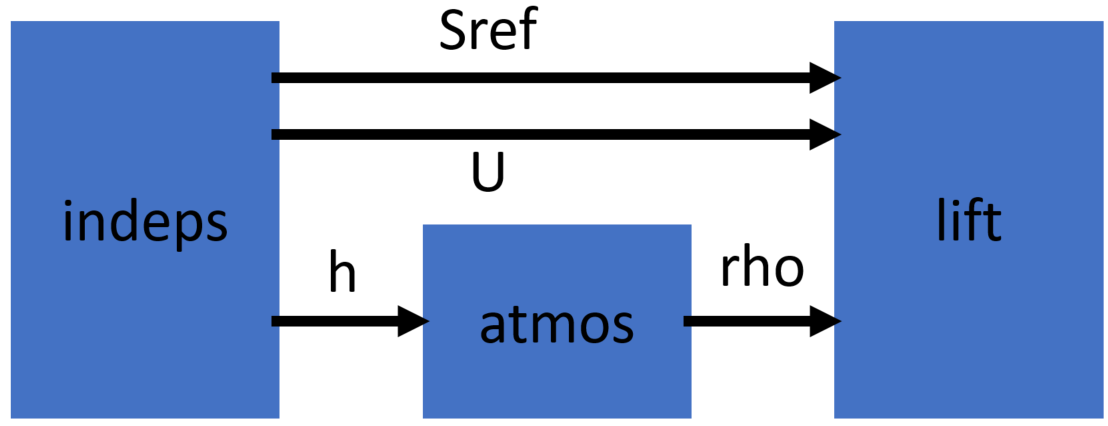
\includegraphics[scale=0.22]{images/explicit_box.png}};
%    }
%
%    \pause %----------------------------------------
%
%    \only<5>{
%        \begin{textblock*}{5cm}(10cm,6cm)
%            \footnotesize \textcolor{red}{Note the namespace / address string\: component\_name.variable}
%        \end{textblock*}
%
%        \tikz[overlay]
%            \draw[red, very thick, <-](6.5,2.6) to (8.5,2.6);
%        \tikz[overlay]
%            \draw[red, very thick, <-](2.65,0.5) to (8.45,2.5);
%    }
%
%    \pause %----------------------------------------
%
%    \only<6>{
%        \begin{tikzpicture}[overlay]
%            % Problem image
%            \node[anchor=center] at ($(current page.center)-(-4.5,-0.5)$)
%            {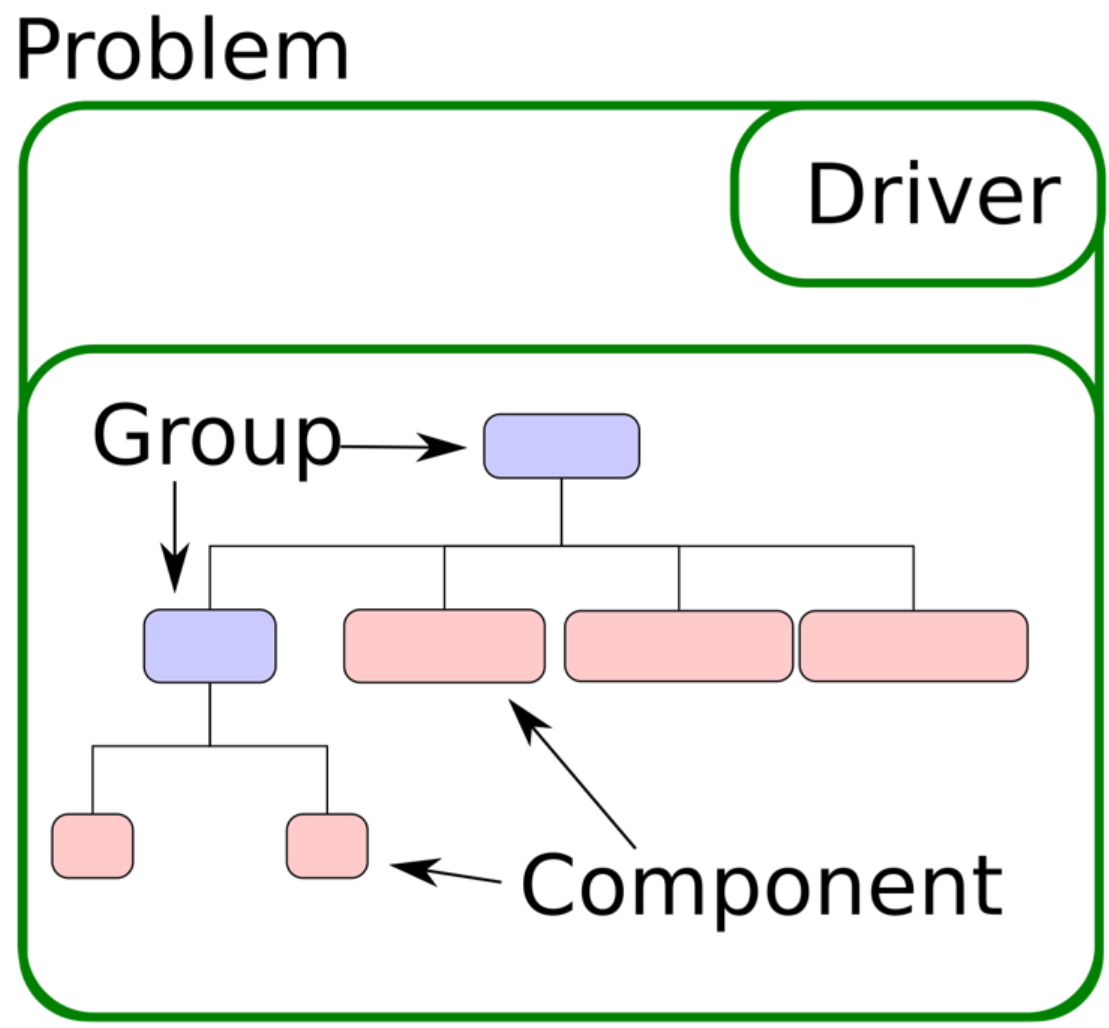
\includegraphics[scale=0.15]{images/arch1.png}};
%
%            % Circle on image
%            \draw [red, ultra thick] (12.55,5.3) circle (0.45cm);
%
%            % Rectangle
%            \draw [red, ultra thick](0.4,2.1) rectangle (5,1.5);              % Format: (x1,y1) rectangle (x2,y2)
%
%            % Dotted line connecting circle and rectangle
%            \draw[dotted, red, ultra thick] (5,2.1) -- (12,5.3);
%        \end{tikzpicture}
%
%        \begin{textblock*}{6cm}(7cm,7.5cm)
%            \footnotesize \textcolor{red}{When you run an MDA/MDO problem, you will add one top-level Group instance to the problem}
%        \end{textblock*}
%    }
%
%\end{frame}
%
%%---------------------------------------------------------------------%
%%---------------------------------------------------------------------%
%
%\begin{frame}{Another way to connect…}
%    \begin{itemize}
%        \item If parameters are widely used among many components, writing many connect() statements can be tedious
%        \item Variable \textit{promotion} is another way to make connections
%    \end{itemize}
%    \vspace{0.75cm}
%
%    % import python source code from file
%    \lstinputlisting[firstline=1, lastline=12, language=Python]{SourceCodes/another_way_to_connect.py}
%
%    % Rectangle at line 11
%    \tikz[overlay]
%        \draw[red, very thick] (6.7,0.8) rectangle (13.5,1.2);
%
%\end{frame}
%
%%---------------------------------------------------------------------%
%%---------------------------------------------------------------------%
%
%\begin{frame}{What does variable promotion do?}
%    \begin{itemize}
%        \item Creates an alias for the variable one level up in the namespace
%            \begin{itemize}
%                \item (atmos.h - h)
%                \item (lift.rho - rho)
%            \end{itemize}
%        \item Automatically connects any matching I/O variable names
%        \item Promote variables with wildcard (e.g. *\_\textcolor{blue}{in} or just *)
%    \end{itemize}
%
%    \lstinputlisting[firstline=1, lastline=12, language=Python]{SourceCodes/another_way_to_connect.py}
%
%    % Rectangle at line 11
%    \tikz[overlay]
%        \draw[red, very thick] (6.7,0.8) rectangle (13.5,1.2);
%
%\end{frame}
%
%%---------------------------------------------------------------------%
%%---------------------------------------------------------------------%
%
%\begin{frame}{What does variable promotion do?}
%    \lstinputlisting[language=Python]{SourceCodes/another_way_to_connect.py}
%
%    \begin{tikzpicture}[overlay]
%        \draw[red, very thick] (8.4,4.9) rectangle (13,5.25);      % Top Box
%        \draw[red, very thick] (8.2,3.05) rectangle (12.9,3.45);    % Middle box
%        \draw [red, ultra thick](0.4,1.1) rectangle (4,1.7);        % Bottom box
%        \node[anchor=center] at ($(current page.center)-(-3,3)$)    % Image
%            {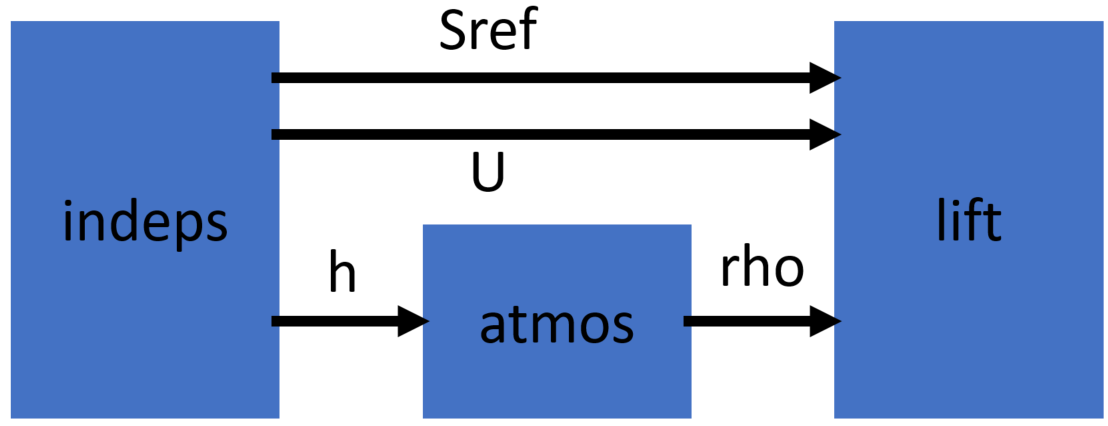
\includegraphics[scale=0.25]{images/explicit_box.png}};
%    \end{tikzpicture}
%
%        \begin{textblock*}{4cm}(10cm,4cm)
%            \footnotesize \textcolor{red}{Input/output connection established automatically}
%        \end{textblock*}
%\end{frame}
%
%%---------------------------------------------------------------------%
%%---------------------------------------------------------------------%
%
%\begin{frame}{What does variable promotion do?}
%    \lstinputlisting[language=Python]{SourceCodes/another_way_to_connect_2.py}
%
%    \only<1>{
%        \begin{textblock*}{5cm}(9cm,2.8cm)
%            \footnotesize \textcolor{red}{Multiple promoted outputs with same name: not allowed (will raise an exception)}
%        \end{textblock*}
%
%        \begin{tikzpicture}[overlay]
%            \draw[red, very thick] (8.2,3.05-0.5) rectangle (12.9,2.95);    % Top box
%            \draw[red, very thick] (8.35,2.05-0.5) rectangle (11.65,1.98);    % Bottom box
%        \end{tikzpicture}
%
%
%    }
%
%    \pause
%
%    \only<2>{
%        \begin{tikzpicture}[overlay]
%            \draw[red, very thick] (8.25,0.5) rectangle (13.1,1.2);    % Top box
%        \end{tikzpicture}
%
%        \begin{textblock*}{6cm}(8cm,7.5cm)
%            \footnotesize \textcolor{red}{Multiple promoted inputs with identical name: OK and encouraged (all connections automatically made)}
%        \end{textblock*}
%
%    }
%
%\end{frame}
%
%%---------------------------------------------------------------------%
%%---------------------------------------------------------------------%
%
%\begin{frame}{What does variable promotion do?}
%    \lstinputlisting[language=Python]{SourceCodes/connecting_multiple_components_2.py}
%
%    \tikz[overlay]
%        \draw[red,very thick, <-] (5.5,.6) to (8,0.15);      % Left Arrow
%    \tikz[overlay]
%        \draw[red, very thick, <-] (10.8,0.9) to (9,0.15);   % Right Arrow
%
%    \begin{textblock*}{5cm}(8.3cm, 7.4cm)
%        \footnotesize \textcolor{red}{Mixing promotion with connect statements:allowed / appropriate}
%    \end{textblock*}
%\end{frame}
%
%%---------------------------------------------------------------------%
%%---------------------------------------------------------------------%
%
%\begin{frame}{Lab 0: Implementing simple explicit calculations (Breguet Range)}
%    \begin{itemize}
%        \item Install OpenMDAO
%        \vspace{0.5cm}
%        \item Write your first component
%        \vspace{0.5cm}
%        \item World domination!
%    \end{itemize}
%
%\end{frame}
%
%%---------------------------------------------------------------------%
%%---------------------------------------------------------------------%
%
%\begin{frame}{Lab 0.a: Install}
%    \begin{itemize}
%        \item Open cmd prompt
%        \vspace{0.25cm}
%        \item Internet install: \texttt{pip install openmdao}
%        \vspace{0.25cm}
%        \item Local Install:
%            \begin{itemize}
%                \item cd to wherever OpenMDAO is downloaded: \texttt{'pip install .'} \textcolor{red}{(note the period)}
%                \item This installs from local source files, not PyPI
%            \end{itemize}
%        \vspace{0.25cm}
%        \item cd ../openmdao\_training
%        \vspace{0.25cm}
%        \item \texttt{\textcolor{red}{python} paraboloid.py}
%            \begin{itemize}
%                \item If this works without error, your installation should be good
%            \end{itemize}
%    \end{itemize}
%\end{frame}
%
%%---------------------------------------------------------------------%
%%---------------------------------------------------------------------%
%
%\begin{frame}{Lab 0.b: Aircraft Range}
%    \begin{itemize}
%        \item Open \texttt{lab\_0\_template.py} in a text editor or IDE and rename it to \texttt{lab\_0.py}
%        % \vspace{0.25cm}
%
%        \item The \texttt{BreguetRange} component implements the electric Breguet equation:
%
%        \begin{equation}
%          \small R_b= \frac{L}{D}\eta_e \eta_int \eta_p \frac{e_b}{g} \frac{m_b}{m_TO}
%        \end{equation}
%        % \vspace{0.1cm}
%
%        \begin{equation}
%          \small m_TO = m_{empty} + m_{payload} + m_{battery}
%        \end{equation}
%        % \vspace{0.1cm}
%
%        \item Your goal is to compute the maximum range of an airplane given a certain payload
%    \end{itemize}
%\end{frame}
%
%%---------------------------------------------------------------------%
%%---------------------------------------------------------------------%
%
%\begin{frame}{Lab 0.b: Aircraft Range}
%    \begin{itemize}
%        \item Complete the TODOs in the \texttt{BatteryWeight} component
%        \vspace{0.3cm}
%        \item Complete the TODOs in the \texttt{ElecRangeGroup} definition by connecting the two components
%        \vspace{0.3cm}
%        \item \texttt{cd} into project folder to check and run the model
%            \begin{itemize}
%                \item \texttt{openmdao view\_model lab\_0.py}  (creates model diagram)
%                \item \texttt{python lab\_0.py}               (runs the model)
%            \end{itemize}
%            \vspace{0.3cm}
%        \item Answer key in the \texttt{lab\_0\_solution.py} file (don’t cheat!)
%    \end{itemize}
%\end{frame}
%
%%---------------------------------------------------------------------%
%%---------------------------------------------------------------------%
%
%\begin{frame}{Lab 0.b: Aircraft Range}
%    \begin{itemize}
%        \item \texttt{openmdao view\_model lab\_0.py}
%        \item If you forgot any connections, you’ll see some red
%    \end{itemize}
%
%    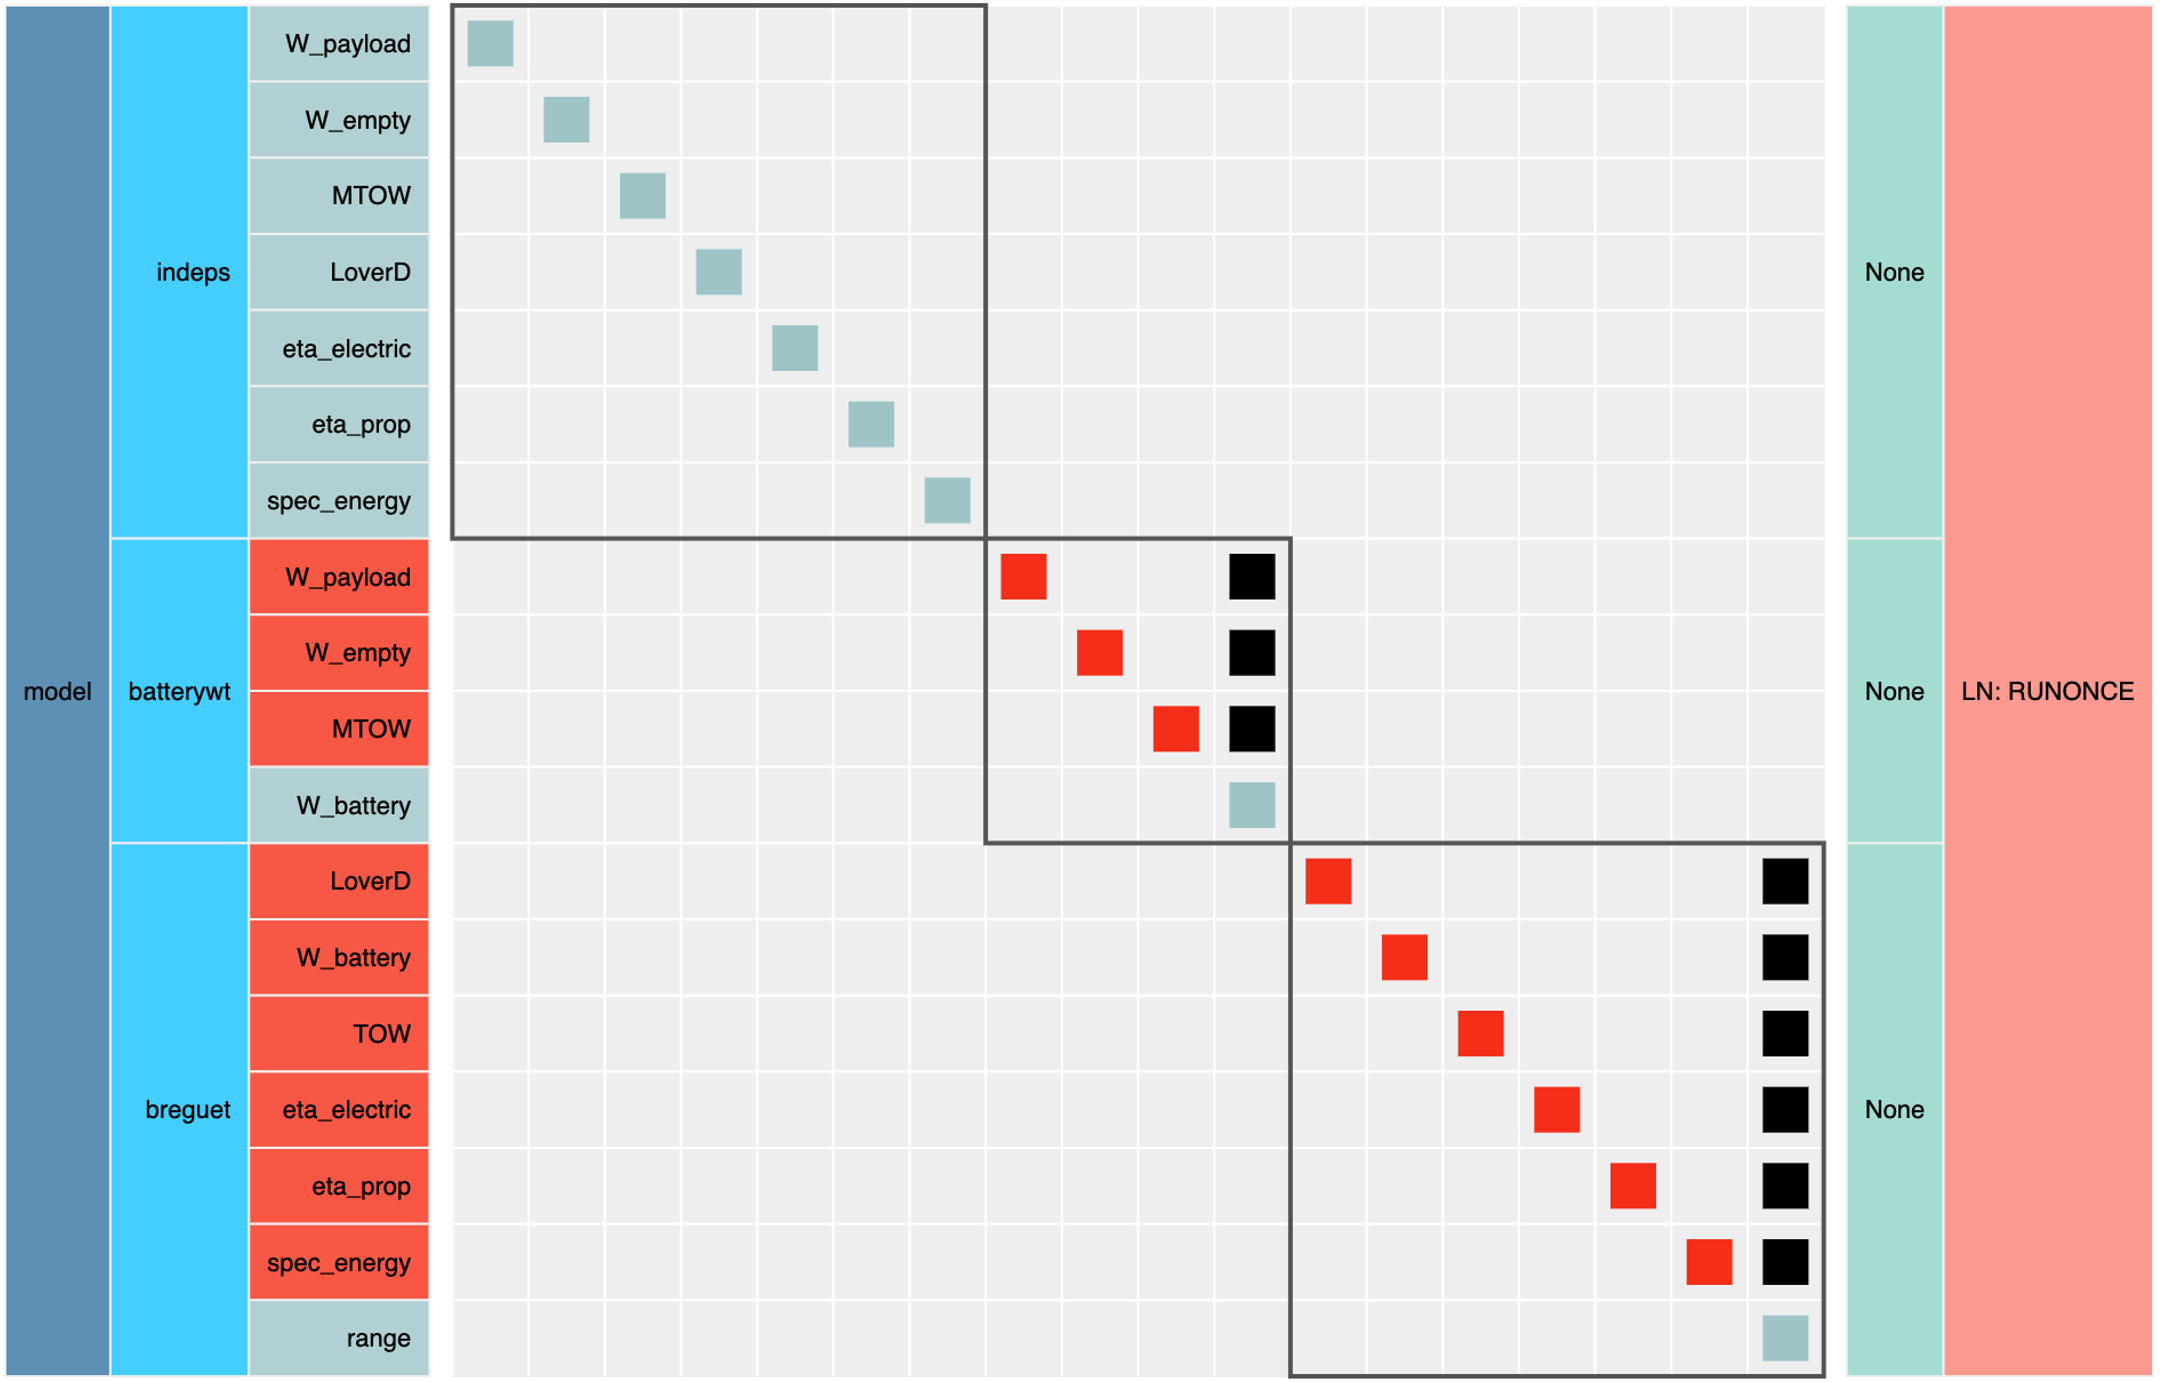
\includegraphics[scale=0.21]{images/lab_0_N2.png}
%
%    \begin{textblock*}{4cm}(11cm,4cm)
%        \small \textcolor{red}{All the red boxes represent unconnected inputs to components.}
%    \end{textblock*}
%
%    \begin{textblock*}{4cm}(11cm,6cm)
%        \small Use explicit connection or variable promotion to get rid of all the red
%    \end{textblock*}
%\end{frame}
%
%%---------------------------------------------------------------------%
%%---------------------------------------------------------------------%
%
%\begin{frame}{Lab 0.b: The n2 is your best friend!}
%    \vspace{1cm}     % Move image down
%
%    % N2 Diagram and the Legend side by side
%    \begin{columns}
%        \column[T]{0.8\textwidth}
%            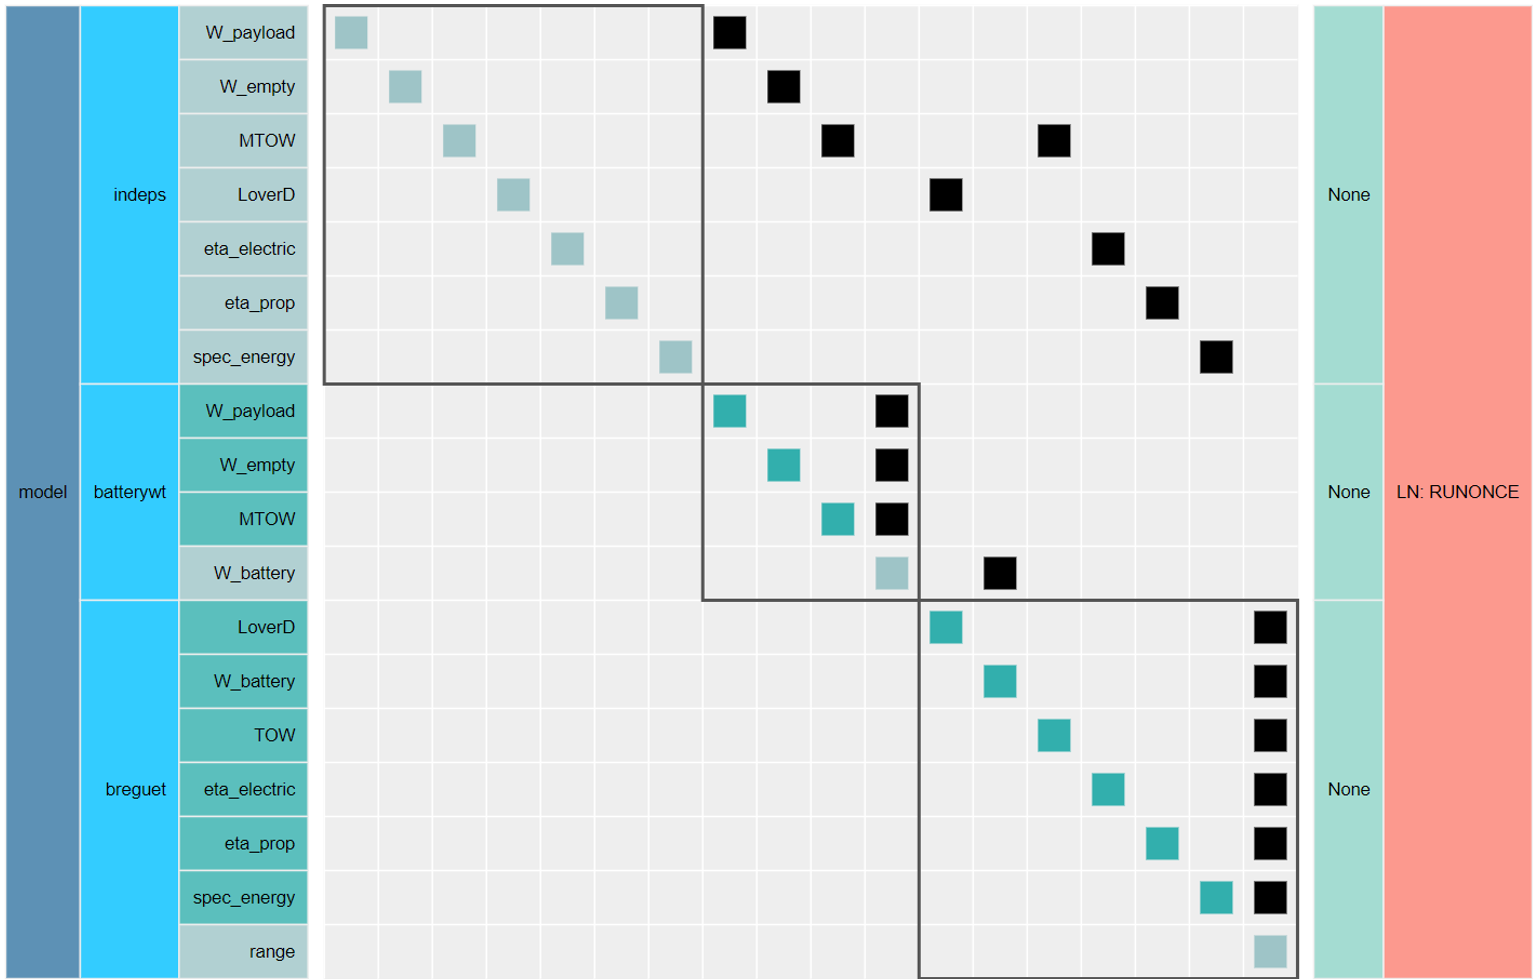
\includegraphics[scale=0.3]{images/n2_48.PNG}  % N2 diagram
%        \column[T]{0.2\textwidth}
%            \hspace{-2cm}
%            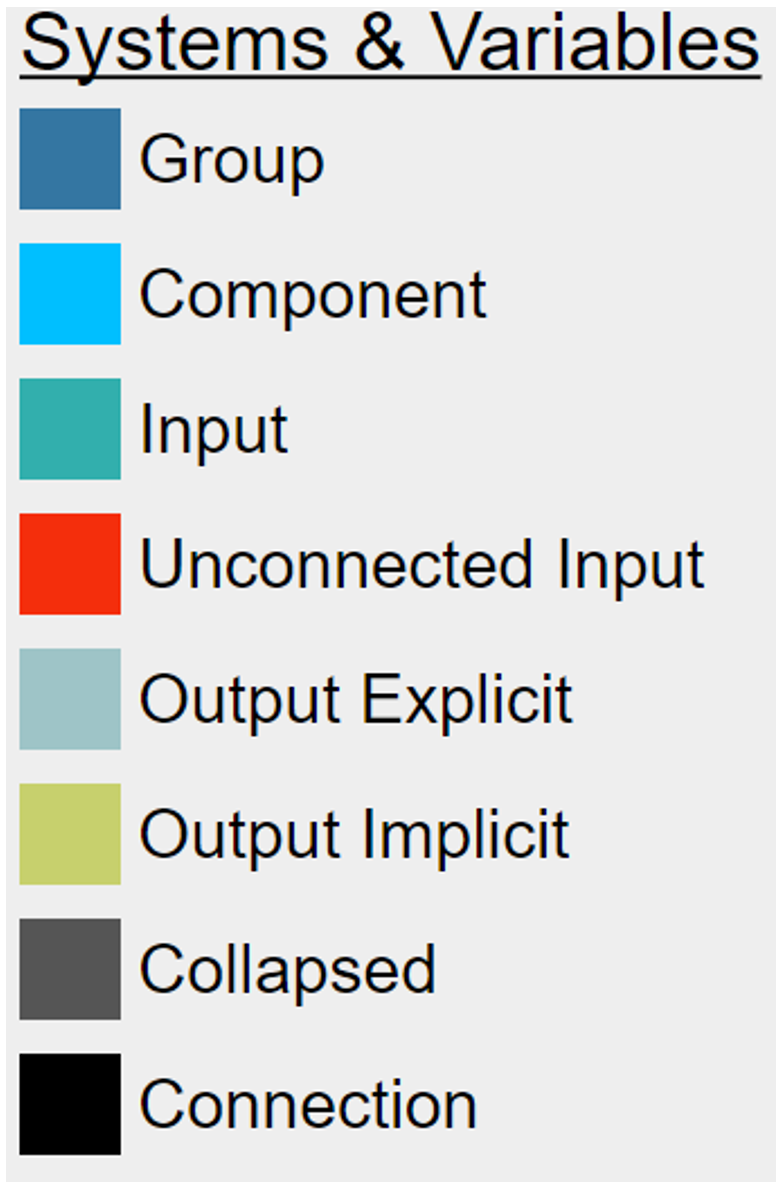
\includegraphics[scale=0.26]{images/n2_legend.png}
%    \end{columns}
%
%    % Begin all text on the frame
%    \begin{textblock*}{4.25cm}(3cm,2.3cm)
%        \footnotesize \textcolor{red}{\textbf{Model hierarchy (groups, components, variables}}
%    \end{textblock*}
%
%    \begin{textblock*}{4cm}(10cm,2.3cm)
%      \footnotesize \textcolor{red}{\textbf{Linear and nonlinear solver hierarchy (more on this later…)}}
%    \end{textblock*}
%
%    \begin{textblock*}{3cm}(3cm,7.5cm)
%      \footnotesize \textcolor{red}{\textbf{Inside a box is within a single component}}
%    \end{textblock*}
%
%    \begin{textblock*}{4cm}(4.6cm,5.3cm)
%        \footnotesize \textcolor{red}{\textbf{Connections!}}        % Top grid-line = 2cm, ++
%    \end{textblock*}
%
%    % Begin all tikzpictures
%    \begin{tikzpicture}[overlay]
%        \draw[red,very thick, <-] (1,5.6) to (1.8,6.3);       %Left arrow
%        \draw[red,very thick, <-] (7.5,5.6) to (8.9,6.3);     % Right arrow
%    \end{tikzpicture}
%
%
%
%\end{frame}
%
%%---------------------------------------------------------------------%
%%---------------------------------------------------------------------%
%
%\begin{frame}{Lab 0.b: Aircraft Range}
%    \begin{columns}
%        \column[T]{0.5\textwidth}
%            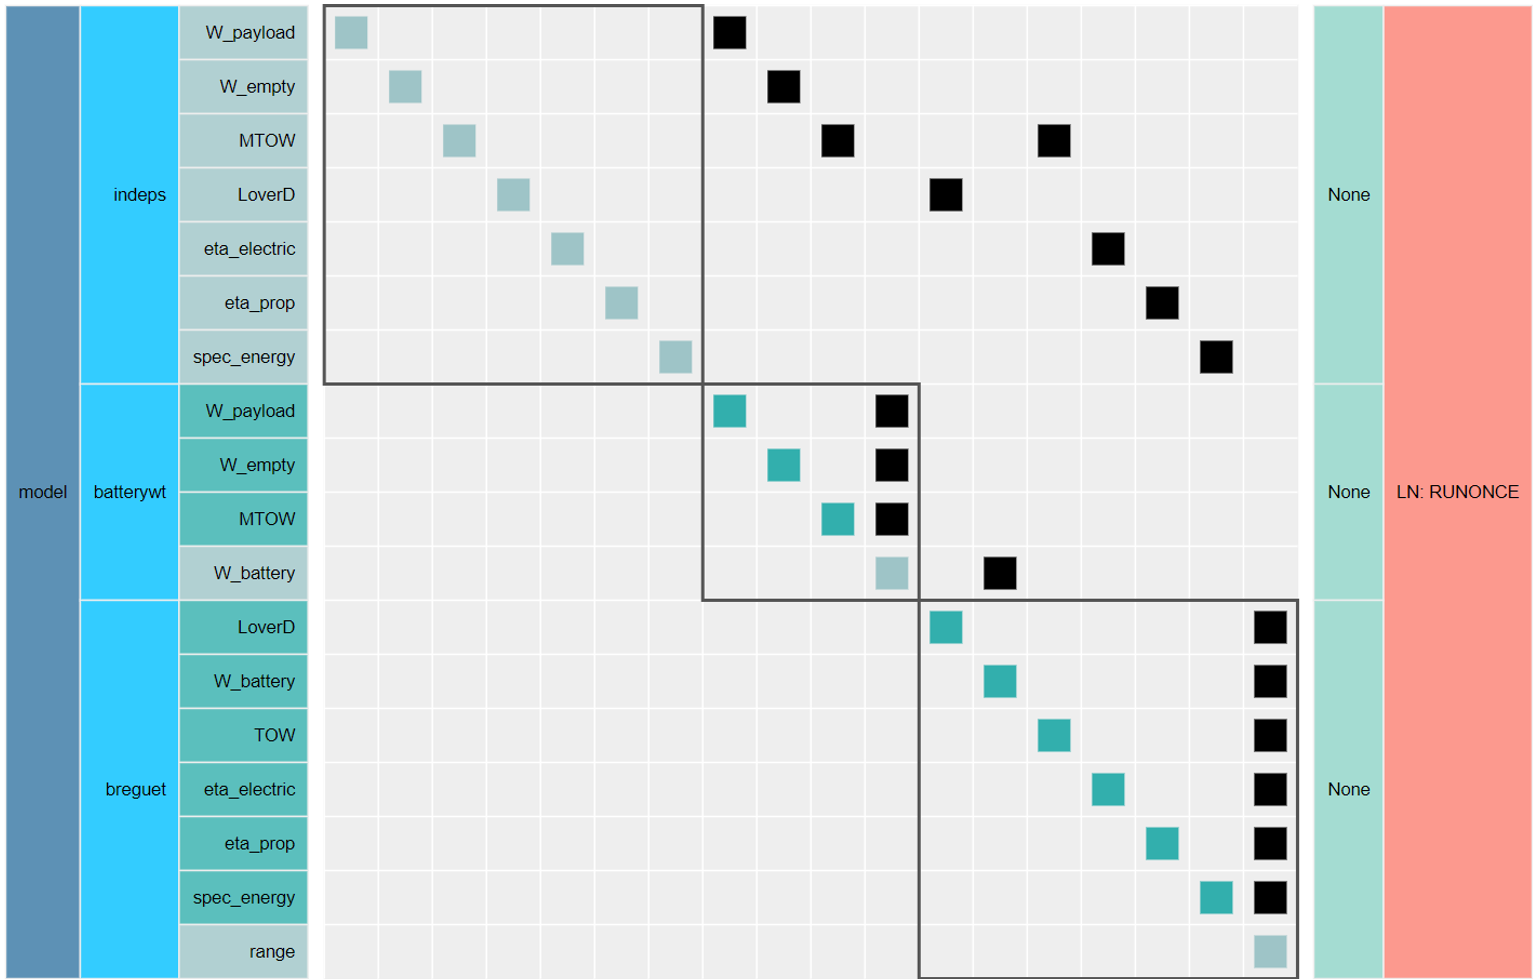
\includegraphics[scale=0.3]{images/n2_48.PNG}\newline   % N2 diagram
%            \footnotesize \textcolor{red}{N2 diagram is upper-triangular:
%            Pure explicit \newline computation (feed-forward)}
%
%        \column[T]{0.4\textwidth}
%            \begin{itemize}
%                \item It should look like this!
%                \vspace{0.5cm}
%                \item \textbf{This diagram is interactive}
%                \vspace{0.5cm}
%                \item Right click on the components/groups to collapse and expand them
%                \vspace{0.5cm}
%                \item Click on any black colored square to trace connections between components
%            \end{itemize}
%    \end{columns}
%\end{frame}         % Error is from the image being outside of the column fram (can ignore)
%
%%---------------------------------------------------------------------%
%%---------------------------------------------------------------------%
%
%\begin{frame}{Lab 0 summary:}
%    \begin{itemize}
%        \item \textit{Everything we just did we can do faster in Excel.}
%        \vspace{0.5cm}
%        \item This is a tutorial so the models are extremely simple and cheap, but …
%        \vspace{0.25cm}
%            \begin{itemize}
%                \vspace{0.25cm}
%                \item Real-world models have hierarchies of dozens or hundreds of logical components
%                \vspace{0.25cm}
%                \item Real-world models often lack a closed form solution and require some kind of solver or iteration strategy
%            \end{itemize}
%    \end{itemize}
%\end{frame}
%
%%---------------------------------------------------------------------%
%%---------------------------------------------------------------------%
%
%\begingroup
%\setbeamercolor{background canvas}{bg=GreenYellow}
%\begin{frame}{Using solvers with implicit models}
%
%    \begin{itemize}
%        \item Gradient-free solver: Nonlinear Block Gauss-Seidel (i.e. Fixed point iteration)
%        \vspace{0.5cm}
%        \item Gradient-based solver: Newton’s Method
%        \vspace{0.5cm}
%        \item Lab 1: Simple aircraft sizing and experimenting with different solver algorithms
%    \end{itemize}
%\end{frame}
%\endgroup
%
%%---------------------------------------------------------------------%
%%---------------------------------------------------------------------%
%
%\begin{frame}{OpenMDAO Nonlinear Solvers}
%    When a circular dependency is detected, OpenMDAO needs a solver to converge the problem:
%
%    \begin{itemize}
%        \item Choice 1: NonlinearBlockGS()
%        \item Choice 2: NewtonSolver()
%        \item Choice 3: BroydenSolver()
%        \item Choice 4: NonlinearBlockJac()
%    \end{itemize}
%\end{frame}
%
%%---------------------------------------------------------------------%
%%---------------------------------------------------------------------%
%
%\begin{frame}{Check out the docs for more info!}
%    \begin{columns}
%        % \vspace{1cm}
%        \column[T]{0.5\textwidth}
%            Look at the docs for OpenMDAO's standard library:
%            \newline
%
%            Lots of details on all the different solvers!
%            \newline
%
%            \uncover<2->{Also see sections for surrogates and helpful general purpose components!}
%
%        \column[T]{0.5\textwidth}
%            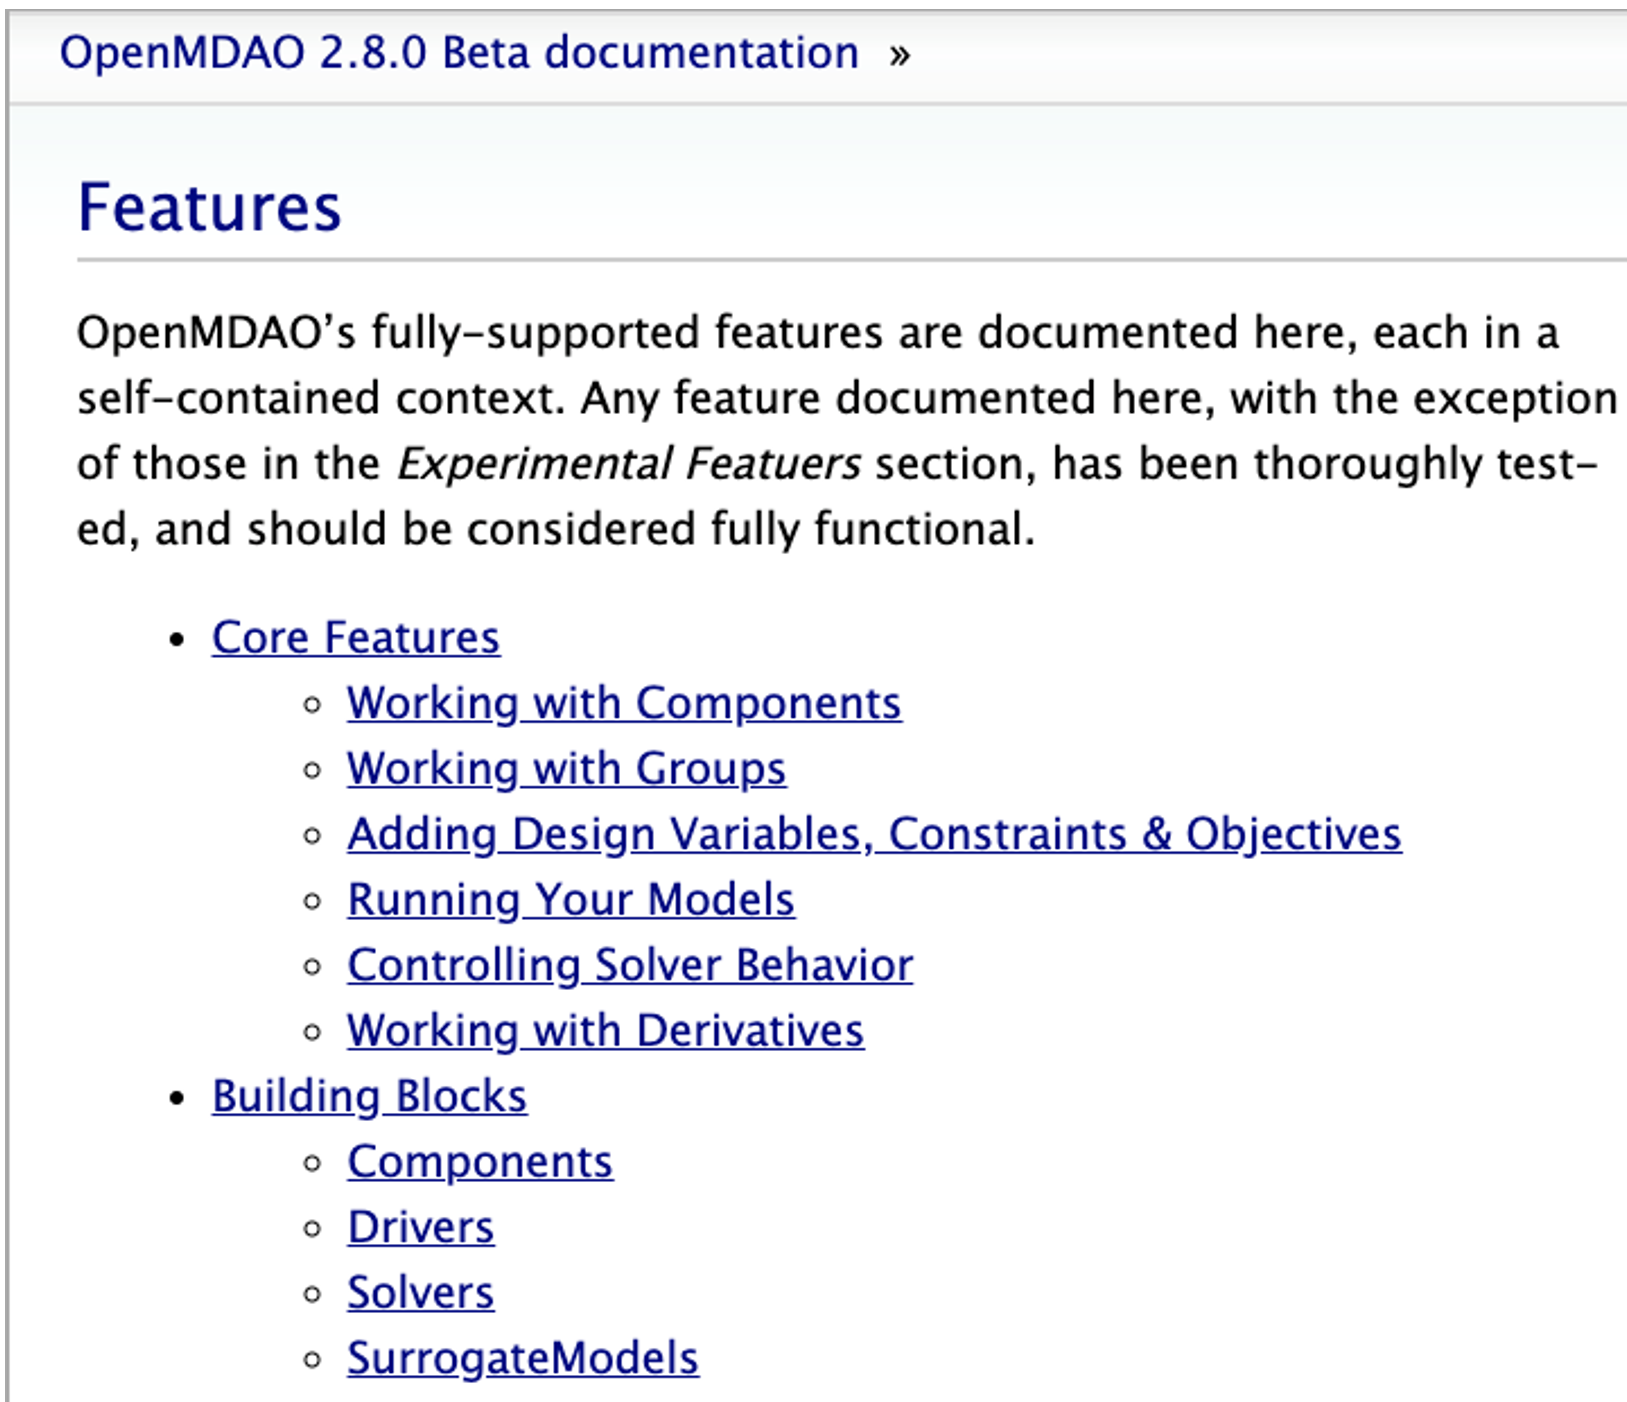
\includegraphics[scale=0.25]{images/documentation_53.png}
%        \end{columns}
%
%        \begin{tikzpicture}[overlay]
%            % Arrow on the first frame
%            \only<1>{\draw[red, very thick, ->](1.5,3.7) to (8.6,0.5);}
%            % Arrows on the second frame
%            \uncover<2->{\draw[red, very thick, ->](4,1.4) to (8.6,1.1);
%                         \draw[red, very thick, ->](4,1.4) to (8.6, 0.25);}
%        \end{tikzpicture}
%\end{frame}
%
%%---------------------------------------------------------------------%
%%---------------------------------------------------------------------%
%
%\begin{frame}{Nonlinear Block Gauss-Seidel}
%    % Setting up tikzpicture for all nodes, the /.style is the formatting for the respective nodes (shapes)
%    \begin{tikzpicture}[overlay,
%        node distance = 0cm and 0.5cm,
%        model/.style = {rectangle, draw, fill=blue!60, minimum width=2cm, minimum height=2cm, align=center},
%        input/.style = {rectangle, draw, fill=blue!20, minimum width=0.75cm, minimum height=0.6cm, align=center}]
%
%        % Large Model Block Nodes (mod#)
%        \node (mod1)  [model, xshift=5cm,     yshift=1.7cm ]   {Model 1};
%        \node (mod2)  [model, below=of mod1,  xshift=2cm   ]   {Model 2};
%        \node (mod3)  [model, below=of mod2,  xshift=2cm   ]   {Model 3};
%
%        % Smaller input nodes on the left side (in#)
%        \node (in1)   [input, left=of mod1,   yshift= 0.7cm     ]   {};
%        \node (in2)   [input, below=of in1,   yshift= -0.066cm  ]   {};
%        \node (in3)   [input, below=of in2,   yshift= -0.066cm  ]   {};
%
%        \uncover<2->{
%            \node (mod1)  [model, xshift=5cm,    yshift= 1.7cm, fill=green!40]   {Model 1};
%            \node (in4)   [input, above=of mod1, yshift= 0.1cm, fill=green!40]   {};
%        }
%
%        \uncover<3->{
%            \node (mod2)  [model, below=of mod1,   xshift= 2cm,       fill=yellow!40 ]  {Model 2};
%            \node (in5)   [input, above=of mod2,   yshift= 0.1cm,     fill=yellow!40 ]  {};
%            \node (in6)   [input, below=of in3,    yshift= -0.066cm,  fill=green!40  ]  {};
%            \node (in7)   [input, below=of in6,    yshift= -0.066cm                  ]  {};
%            \node (in8)   [input, below=of in7,    yshift= -0.066cm                  ]  {};
%        }
%
%        \uncover<4->{
%            \node (mod3)   [model, below=of mod2,  xshift= 2cm,       fill=orange!50 ]   {Model 3};
%            \node (in9)    [input, above=of mod3,  yshift= 0.1cm,     fill=orange!50   ]   {};
%            \node (in10)   [input, below=of in8,   yshift= -0.066cm,  fill=green!40  ]   {};
%            \node (in11)   [input, below=of in10,  yshift= -0.066cm,  fill=yellow!40 ]   {};
%            \node (in12)   [input, below=of in11,  yshift= -0.066cm                  ]   {};
%        }
%
%        \uncover<5->{
%            \node (mod1)  [model, xshift=5cm,     yshift=1.7cm,       fill=red!10     ]   {Model 1};
%            \node (in1)   [input, left=of mod1,   yshift= 0.7cm,      fill=green!70   ]   {};
%            \node (in2)   [input, below=of in1,   yshift= -0.066cm,   fill=yellow!70  ]   {};
%            \node (in3)   [input, below=of in2,   yshift= -0.066cm,   fill=orange!70  ]   {};
%            \node (in4)   [input, above=of mod1,  yshift= 0.1cm,      fill=red!10     ]   {};
%        }
%
%        \uncover<6->{
%            \node (mod2)  [model, below=of mod1,   xshift= 2cm,       fill=green!70  ]  {Model 2};
%            \node (in5)   [input, above=of mod2,   yshift= 0.1cm,     fill=green!70  ]  {};
%            \node (in6)   [input, below=of in3,    yshift= -0.066cm,  fill=red!10    ]  {};
%            \node (in7)   [input, below=of in6,    yshift= -0.066cm,  fill=yellow!70 ]  {};
%            \node (in8)   [input, below=of in7,    yshift= -0.066cm,  fill=orange!70 ]  {};
%
%        }
%
%        % line and arrow connecting Model 3 to the input, Only on frame 1
%        \only<1>{
%            \draw [blue, very thick] (mod3) -- (2,-2.3);
%            \draw [blue, very thick] (2,-2.3) -- (2,1.05);
%            \draw [blue, very thick, ->] (2,1.05) -- (in3);
%        }
%    \end{tikzpicture}
%
%% Text Blocks -------------------------------------------
%    \begin{textblock*}{2cm}(13cm,3cm)
%        \textbf{\textcolor{red}{Outputs}}
%    \end{textblock*}
%
%    \begin{textblock*}{3cm}(1cm,5cm)
%        \footnotesize \textcolor{red}{\textbf{Inputs}}
%    \end{textblock*}
%
%    \only<1>{
%        % Text describing the connection arrow
%        \begin{textblock*}{3cm}(5cm,7cm)
%            \textcolor{red}{Cycle connection}
%        \end{textblock*}
%    }
%
%    \only<1,2>{
%        % Text on left side
%        \begin{textblock*}{3cm}(1cm,5.5cm)
%            \footnotesize \textcolor{red}{Initial guess}
%        \end{textblock*}
%    }
%
%    \only<2>{
%        % Text next to Model 1 block
%        \begin{textblock*}{5cm}(7.5cm,3cm)
%            \small \textcolor{red}{Evaluate Model 1 using initial guess inputs }
%        \end{textblock*}
%    }
%
%    \only<3>{
%        % Text next to Model 2 block
%        \begin{textblock*}{5cm}(9.5cm,5cm)
%            \small \textcolor{red}{Substitute Model 1 output into state vector and run Model 2
%}
%        \end{textblock*}
%    }
%
%    \only<4>{
%        % Text next to Model 3 block
%        \begin{textblock*}{4.3cm}(11.3cm,7cm)
%            \small \textcolor{red}{Substitute Model 2 output into state vector and run Model 3}
%        \end{textblock*}
%    }
%
%    \only<5>{
%        % Text next to Model 1 block
%        \begin{textblock*}{5cm}(7.5cm,2.5cm)
%            \footnotesize \textcolor{red}{Run Model 1 with input from all prior tools. Repeat until converged}
%        \end{textblock*}
%    }
%
%        \only<6>{
%        % Text next to Model 1 block
%        \begin{textblock*}{5cm}(7.5cm,2.5cm)
%            \footnotesize \textcolor{red}{Run Model 2 with input from all prior tools. Repeat until converged}
%        \end{textblock*}
%    }
%
%\end{frame}
%
%%---------------------------------------------------------------------%
%%---------------------------------------------------------------------%
%
%\begin{frame}{\small Newton’s Method is simple in one dimension (Gradient Based!)}
%    \begin{columns}
%        \column[T]{0.5\textwidth}
%            \begin{equation}
%                x_{n+1} = x_{n} - \frac{f(x_{n})}{f'(x_{n})}                    % Equation
%            \end{equation}
%
%        \column[T]{0.5\textwidth}
%        \begin{tikzpicture}
%            \draw       [black, very thick]     (0,-0.5) parabola (5,3);        % parabola
%            \draw       [black, thick, ->]      (0,0) to (6,0);                 % X-axis
%            \draw       [blue, thin]            (2.6, 0) -- (5.4, 3.3);         % Intersection line
%            \draw       [blue, ->]              (4.5, 2.3) to (4.5, 0);         % Xn arrow
%            \filldraw   [red]                   (4.5,2.3) circle (0.15cm);      % Top red circle
%            \filldraw   [red]                   (2.6,0) circle (0.15cm);        % Lower red circle
%        \end{tikzpicture}
%
%    \end{columns}
%
%    % Begin text blocks
%    \begin{textblock*}{3cm}(10cm, 3.5cm)
%        \small \textcolor{red}{Slope = $f'(x_{n})$}
%    \end{textblock*}
%
%    \begin{textblock*}{3cm}(13cm, 5.5cm)
%        \small \textcolor{red}{$f'(x_{n})$}
%    \end{textblock*}
%
%    \begin{textblock*}{3cm}(12.8cm, 7.15cm)
%        \small \textcolor{red}{$x_{n}$}
%    \end{textblock*}
%
%    \begin{textblock*}{3cm}(11cm, 7.15cm)
%        \small \textcolor{red}{$x_{n+1}$}
%    \end{textblock*}
%\end{frame}
%
%%---------------------------------------------------------------------%
%%---------------------------------------------------------------------%
%
%%\begin{frame}{Newton Solver for multiple dimensions is a bit more complex}
%%    % Matrix representations on left side of frame
%%    \begin{columns}
%%    \column[C]{0.25\textwidth}
%%        \vspace{-7cm}
%%        \begin{tikzpicture}[overlay,
%%            node distance = 0cm and 0.1cm,
%%            big/.style = {rectangle, draw, fill=blue!60, minimum width=1.5cm, minimum height=1.5cm, align=center},
%%            small/.style = {rectangle, draw, fill=blue!60, minimum width=0.5cm, minimum height=1.5cm,    align=center},
%%            txt/.style={}]
%%
%%            Note: location of the node matters!
%%            \node (big1)    [big, xshift=.6cm,   yshift= 0cm]   {};
%%            \node (small1)  [small, right=of big1           ]   {};
%%            \node (textA)   [txt,  above=of big1           ]   {\textcolor{red}{$n_{y}$}};
%%            \node (textB)   [txt,  left= of big1           ]   {\textcolor{red}{$n_{y}$}};
%%            \node (text_eq) [txt,  right=of small1         ]   {\textbf{\textcolor{red}{=}}};
%%            \node (small2)  [small, right=of text_eq        ]   {};
%%            \node (textC)   [txt,  above=of small1         ]   {\textcolor{red}{1}};
%%            \node (textD)   [txt,  above=of small2         ]   {\textcolor{red}{1}};
%%            \node (textE)   [txt, right=of small2          ]   {\textcolor{red}{$n_{y}$}};
%%        \end{tikzpicture}
%%
%%    \column[T]{0.33\textwidth}
%%    \hspace{-1cm}
%%    \begin{small}
%%        \begin{equation*}
%%            R(x,y)=0
%%        \end{equation*}
%%        \begin{equation*}
%%          \hspace{-1cm} R(x,y + \delta y) = R(x,y) + \frac{\partial R}{\partial y} \delta y + HOT
%%        \end{equation*}
%%        \begin{equation*}
%%            0 = R(x,y) + \frac{\partial R}{\partial y} \delta y
%%        \end{equation*}
%%        \begin{equation*}
%%            \delta y = -\frac{\partial R^{-1}}{\partial y}R(x,y)
%%        \end{equation*}
%%        \begin{equation*}
%%            \frac{\partial R}{\partial y} \delta y = -R(x,y)
%%        \end{equation*}
%%        \begin{equation*}
%%          y_{n+1} = y_{n} + \delta y
%%        \end{equation*}
%%    \end{small}
%%
%%
%%    \column[T]{0.33\textwidth}
%%        % Red circle around equation
%%        \tikz[overlay]
%%            \draw [red, very thick] (-3.2cm, -5cm) ellipse (2cm and 0.7cm);
%%
%%    % Begin the text descriptions of each equation
%%        \only<1>{
%%            \begin{textblock*}{5.5cm}(10cm, 6cm)
%%                \small \textcolor{red}{Drive residuals to 0 x: design variables y: implicit state variables}
%%            \end{textblock*}
%%            \tikz[overlay]
%%                \draw [red, very thick, ->] (1.9,-0.25) to (-2cm, -0.25);
%%        }
%%
%%        \only<2>{
%%            \begin{textblock*}{5.5cm}(10cm, 6cm)
%%                \small \textcolor{red}{Do a Taylor series with respect to the current point}
%%            \end{textblock*}
%%            \tikz[overlay]
%%                \draw [red, very thick, ->] (2.9,-1.25) to (0.25cm, -1.25);
%%        }
%%
%%        \only<3>{
%%            \begin{textblock*}{5.5cm}(10cm, 6cm)
%%                \small \textcolor{red}{We want residuals to be 0 at the next iteration y + dy}
%%            \end{textblock*}
%%            \tikz[overlay]
%%                \draw [red, very thick, ->] (2.9,-2.5) to (-1cm, -2.5);
%%        }
%%
%%        \only<4>{
%%            \begin{textblock*}{5.5cm}(10cm, 6cm)
%%                \small \textcolor{red}{Solve for dy that would drive the linearize residuals to 0}
%%            \end{textblock*}
%%            \tikz[overlay]
%%                \draw [red, very thick, ->] (-0.8,-3.6) to (-1.2cm, -3.6);
%%        }
%%
%%        \only<5>{
%%            \begin{textblock*}{5.5cm}(10cm, 6cm)
%%                \small \textcolor{red}{But we don’t actually invert. Just solve this linear system}
%%            \end{textblock*}
%%            \tikz[overlay]
%%                \draw [red, very thick, ->] (1,-5) to (-1cm, -5);
%%        }
%%
%%        \only<6>{
%%            \begin{textblock*}{5.5cm}(10cm, 6cm)
%%                \small \textcolor{red}{Then take a step. Repeat from top until converged}
%%            \end{textblock*}
%%            \tikz[overlay]
%%                \draw [red, very thick, ->] (1,-6) to (-1.5cm, -6);
%%        }
%%
%%    \end{columns}
%%
%%\end{frame}
%
%\begin{frame}{Newton Solver needs some partial derivatives! }
%
%    % Matrix representations on left side of frame
%    \vspace{1cm}
%    \begin{centering}
%        \begin{tikzpicture}[overlay,
%            node distance = 0cm and 0.1cm,
%            big/.style = {rectangle, draw, fill=blue!60, minimum width=1.5cm, minimum height=1.5cm, align=center},
%            small/.style = {rectangle, draw, fill=blue!60, minimum width=0.5cm, minimum height=1.5cm,    align=center},
%            txt/.style={}]
%
%            % Note: location of the node matters!
%            \node (big1)    [big, xshift=6cm ]   {};
%            \node (small1)  [small, right=of big1          ]   {};
%            \node (textA)   [txt,  above=of big1           ]   {\textcolor{red}{$n_{y}$}};
%            \node (textB)   [txt,  left= of big1           ]   {\textcolor{red}{$n_{y}$}};
%            \node (text_eq) [txt,  right=of small1         ]   {\textbf{\textcolor{red}{=}}};
%            \node (small2)  [small, right=of text_eq       ]   {};
%            \node (textC)   [txt,  above=of small1         ]   {\textcolor{red}{1}};
%            \node (textD)   [txt,  above=of small2         ]   {\textcolor{red}{1}};
%            \node (textE)   [txt, right=of small2          ]   {\textcolor{red}{$n_{y}$}};
%        \end{tikzpicture}
%        \end{centering}
%
%    \begin{centering}
%        \vspace{1cm}
%        \begin{equation*}
%            \frac{\partial R}{\partial y} \delta y = -R(x,y)
%        \end{equation*}
%
%        \begin{equation*}
%          y_{n+1} = y_{n} + \delta y
%        \end{equation*}
%    \end{centering}
%
%    \begin{tikzpicture}[overlay]
%        \draw[red, very thick]      (5,2.5) rectangle (5.8,4);    % Red box
%        \draw[red, very thick, ->]  (5.5, 4)   to (5.7, 4.8);     % Left arrow
%        \draw[red, very thick, ->]  (6.2, 3.5) to (7, 4.8);       % Middle arrow
%        \draw[red, very thick, ->]  (8, 3.5)   to (8.6, 4.8);     % Right arrow
%    \end{tikzpicture}
%
%\end{frame}
%
%\begin{frame}{Partial Derivatives in OpenMDAO}
%    \lstinputlisting[language=Python]{SourceCodes/Partial_Derivatives_in_OpenMDAO.py}
%
%
%
%
%
%\end{frame}





\end{document}
